% \documentclass[conference,compsoc]{IEEEtran}
\documentclass{sig-alternate-05-2015}                

% \usepackage[dvipdfmx]{graphicx} \usepackage{amssymb} \usepackage{multirow} \usepackage{threeparttable} \usepackage{array} \usepackage{color} \usepackage{nidanfloat}
\usepackage{graphicx} \usepackage{amssymb} \usepackage{multirow} \usepackage{threeparttable} \usepackage{array} \usepackage{color} \usepackage{nidanfloat}\usepackage{setspace} 


% \author{\IEEEauthorblockN{Yuya Maruyama}\IEEEauthorblockA{School of Engineering Science\\Osaka University}\and\IEEEauthorblockN{Shinpei Kato}\IEEEauthorblockA{Graduate School of Information Science\\Nagoya University}\and\IEEEauthorblockN{Takuya Azumi}\IEEEauthorblockA{Graduate School of Engineering Science\\Osaka University }}

\numberofauthors{2}
\author{
% 1st. author
\alignauthor Yuya Maruyama\\
\affaddr{Graduate School of Engineering Science}\\
\affaddr{Osaka University}\\
       % \affaddr{Institute for Clarity in Documentation}\\
       % \affaddr{1932 Wallamaloo Lane}\\
       % \affaddr{Wallamaloo, New Zealand}\\
       % \email{trovato@corporation.com}
% 2nd. author
% \alignauthor Shinpei Kato\\
% \affaddr{Graduate School of Information Science and Technology}\\
% \affaddr{The University of Tokyo}\\
       % \affaddr{P.O. Box 1212}\\
       % \affaddr{Dublin, Ohio 43017-6221}\\
       % \email{webmaster@marysville-ohio.com}
% 3rd. author
\alignauthor Takuya Azumi\\
\affaddr{Graduate School of Engineering Science}\\
\affaddr{Osaka University}\\
}


% Copyright
%\setcopyright{acmcopyright}
%\setcopyright{acmlicensed}
%\setcopyright{rightsretained}
%\setcopyright{usgov}
%\setcopyright{usgovmixed}
%\setcopyright{cagov}
%\setcopyright{cagovmixed}


%% % DOI
%% \doi{10.475/123_4}

%% % ISBN
%% \isbn{123-4567-24-567/08/06}

%% %Conference
%% \conferenceinfo{EMSOFT '16}{October 2--7, 2016, Pittsburgh, PA, USA}

%% \acmPrice{\$15.00}

%
% --- Author Metadata here ---
% \conferenceinfo{WOODSTOCK}{'97 El Paso, Texas USA}
%\CopyrightYear{2007} % Allows default copyright year (20XX) to be over-ridden - IF NEED BE.
%\crdata{0-12345-67-8/90/01}  % Allows default copyright data (0-89791-88-6/97/05) to be over-ridden - IF NEED BE.
% --- End of Author Metadata ---

\title{Exploring Data Transfer and Parallelization with NoC based Many-Core Processors}
\begin{document}

%% ACM copyright information
\CopyrightYear{2016}
\setcopyright{othergov}
\conferenceinfo{EMSOFT'16,}{October 01-07, 2016, Pittsburgh, PA, USA}
\isbn{978-1-4503-4485-2/16/10}\acmPrice{\$15.00}
\doi{http://dx.doi.org/10.1145/2968478.2968502}

\maketitle

\setcounter{topnumber}{5}%    ページ上部の図表は 5 個まで
\def\topfraction{1.00}%       ページの上 1.00 まで図表で占めて可
\setcounter{bottomnumber}{5}% ページ下部の図表は 5 個まで
\def\bottomfraction{1.00}%    ページの下 1.00 まで図表で占めて可
\setcounter{totalnumber}{10}% ページあたりの図表は 10 個まで
\def\textfraction{0.00}%      ページうち本文が占める割合の下限

% \setlength\textfloatsep{18pt}%  between figure and text
% \setlength\abovecaptionskip{4pt}% between figure and caption
% \setlength\floatsep{18pt}% between figures

\begin{abstract}
The evolution of a next generation computing platform oriented toward multi/many cores is inevitable because the demand for high-performance computation with reasonable power consumption even in embedded real-time systems is increasing.
The Multi-Purpose Processing Array 256 developed by Kalray is a many-core processor platform that includes 256 general-purpose cores with high energy efficiency.
The clusters of the cores share a local memory, and a DMA-capable network-on-chip (NoC) connects the clusters.
In this paper, we investigate and characterize currently achievable data transfer methods of cutting-edge many-core technologies based on NoC.
% The cores communicate with each other by NoC parallelly to manage numerous tasks and optimize the potential of this architecture.
Previous studies have not quantitatively examined the transport latencies nor have they clarified the potential and constraints for low-latency many-core computing.
To address this problem, we illustrate evaluations of end-to-end latencies and the calculation potential of many-core computing with parallel data transfer.
Our experimental results will allow system designers to choose appropriate data transfer methods based on the requirements of their latency-sensitive many-core applications as opposed to just intuitive expectations.
By highlighting many-core computing capabilities, we explore the performance characteristics of currently achievable data transfer methods for many-core computing based on NoC.
\end{abstract}

\keywords{Many-core; Multicore; Network-on-Chip (NoC); Parallelization; Embedded software}


\section{Introduction}
The evolution of a next generation computing platform oriented toward multi/many cores is unavoidable to satisfy the demand for increasing computation in conjunction with reasonable power consumption.
Recently, the computational ability of single core processors has reached its limit and thus the applicability of Moore's law \cite{moore2006cramming} is unclear.
Multi/many core architecture is an important trend in recent years as it integrates cores to realize high-performance and general-purpose computing with low power consumption.
Hence, high energy efficiency is a superior feature of multi/many core platforms.

 As detailed in the preceding paragraph, the demand for increasing computation in conjunction with reasonable power consumption drives the need for multi/many core architecture in several domains.
Real-time embedded systems are an example in which multi/many core platforms are adapted since they face increasing processing requirements.
Extant studies have examined numerous applications of multi/many cores platforms \cite{becker2016contention}, \cite{saidi2015shift}, \cite{perret2016temporal}, \cite{perret2016mapping}, \cite{becker2014mapping}.

For example, automotive systems involve various applications and are sometimes characterized by demands for high-performance computing.
Automotive applications are responsible for several control systems such as the powertrain, chassis, steering wheel, driver assistance and user interface.
Advanced driver assistance systems are
characterized by increasing complexity and computational requirements and necessitate intelligence such as an autonomous driving system.
Moreover, they also require significant energy efficiency and cost reduction.
Although modern automotive systems are composed of several Electronic Control Unit (ECU) managing subsystems,
there is a shift from numerous scattered ECUs to hierarchical multi/many core Domain Controllers (DC).
Evidently, a hybrid scenario is also applicable. 
Specifically, DCs combine performance with low power consumption to realize high parallel processing and efficient data transport.
Furthermore, flexible scalability of a many-core platform acilitates development efficiency.

A related example involves avionics systems that also include various applications and require cost efficiency.
Multi/many core platforms can be applied in the avionics domain due to their highly integrated characteristics and increasing processing demands.
Low power consumption of cores leads to lower cooling requirements, and this is a critical issue for avionics.
Multi/many core platforms reduce energy consumption as well as the costs and weight.
Weight reduction is the most important factor for avionics, and integration with a multi/many core platform reduces the amount of processing boards and cooling units.
Thus, the utilization of an integrated platform results in space, weight and cost reductions.

Hence, multi/many core platforms are fabricated and released as commercial off-the-shelf (COTS) multicore components.
Increasing research attention has focused on multi/many core platforms.
The Multi-Purpose Processing Array (MPPA) 256 developed by Kalray \cite{de2013distributed}, \cite{de2013clustered}, \cite{de2014time}, Single-chip Cloud Computer (SCC) developed by Intel \cite{baron2010single}, and Tile64 developed by Tilera \cite{bell2008tile64} include the clustering of many-core architectures in which cores are mapped closely.
The clusters of cores are capable of performing separate independent applications with respect to the desired power envelope of embedded applications.
Kalray's MPPA-256 packs 256 general-purpose cores.
This significantly exceeds the number of cores in other COTS, and it targets embedded systems, high-performance computing (HPC), image processing, and networking due to the high-performance per watt.
Intel's Xeon Phi \cite{chrysos2014intel}, \cite{chrysos2012intel} is an HPC accelerator.
Xeon Phi and SCC are based on x86 architecture and its targeted use corresponds to data centers and workstations.

Despite the emergence of the need for multi/many core platforms, several difficulties persist in the adaptation of these platforms to real-time embedded systems \cite{becker2016contention}, \cite{saidi2015shift}.
These difficulties are caused by the hardware architecture and strict requirements of embedded systems.
A difficulty involves the sharing of numerous resources (e.g. memory subsystems and I/O devices) by cores. Parallelized complex processes share some resources, and this leads to the frequent occurrence of conflicts.
Cache coherency is also a critical problem owing to their numerous cores.
These difficulties disturb predictable timing behavior and software analysis.
Thus, the timing requirement of real-time embedded systems continues to warrant solutions.
The impact of integrating real-time applications in multi/many core platforms, is not completely understood to date.
This is a critical issue because embedded systems have requirements for reliable and predictable behavior.

\textbf{Contributions:}
This study focuses on examining the performance characteristics of currently achievable data transfer methods for many-core computing based on network-on-chips (NoC), such as MPPA-256, while examining parallel data transfer methods.
We reveal the advantages and disadvantages of many-core computing based on NoC in a quantitative way by leading the following contributions:
\begin{itemize}
\item The evaluations of the data transfer on DMA-capable NoC quantitatively characterize the end-to-end latencies, which depend on the routing and DMA configurations.
\item The scalability of parallelization in many-core processors based on NoC is observed in evaluations of matrix calculations in several situations and a real complex application as a part of an autonomous driving system.
\item The evaluations of the parallel processing examine the characteristics of the memory access speed which varies according to where data is allocated and what accesses the memory.
\end{itemize}

To the best of our knowledge, this is the first study that examines data transfer matters for many-core computing beyond an intuitive expectation to allow system designers to choose appropriate data transfer methods based on the requirements of their latency-sensitive many-core applications.
It is expected that the findings of this study will potentially be applicable to several types of many-core architectures as opposed to just MPPA-256.
Therefore, the contributions of this study can be used in low-latency many-core computing.

\textbf{Organization:}
The remainder of this study is organized as follows.
First, the system model considered in this study is discussed in Section \ref{sec:system_model} in which the hardware model, namely Kalray MPPA-256 Bostan, and the system model are presented.
Second, Section \ref{sec:evaluations} illustrates experimental evaluations.
Subsequently, Section \ref{sec:related work} examines related studies that focus on multi/many core systems.
Finally, Section \ref{sec:conclusion} presents the conclusions and directions for future research.


\section{System Model}
\label{sec:system_model}
This section presents the system model used throughout the study.
The many-core model of Kalray MPPA-256 Bostan is considered.
First, a hardware model is introduced in Section \ref{sec:hardware_model}, and this is followed by a software model in Section \ref{sec:software_model}.

\subsection{Hardware Model}
\label{sec:hardware_model}
The MPPA-256 processor is based on an array of compute clusters (CCs) and I/O subsystems (IOSs) that are connected to nodes of Network-on-Chip (NoC) with a toroidal 2D topology 
(as shown in Figures \ref{fig:mppa_architecture}, \ref{fig:cc_architecture}, and \ref{fig:noc_map}).
The MPPA MANYCORE chip integrates 16 compute clusters and 4 IOS on NoC.
The architecture of Kalray MPPA-256 is presented in this section.

\subsubsection{I/O Subsystems (IOS)}
\label{sec:ios}
MPPA-256 has the following four I/O subsystems (IOSes): North, South, East, and West IOSes.
The North and South IOSes are connected to a DDR interface and an eight-lane PCIe controller.
The East and West IOSes are connected to a quad 10Gb/s Ethernet controller.
Two pairs of IOSes organize two I/O clusters (IOCs) as shown in Figure \ref{fig:mppa_architecture}.

Each IOS comprises of quad IO cores and a NoC interface.
\begin{itemize}
\item \textbf{IO cores}: IO cores are connected to a 16-banked parallel shared memory with a total capacity (IO SMEM) of 2MB, as shown in the left side of Figure \ref{fig:mppa_architecture},
The four IO cores have their own instruction cache 8-way associative corresponding to 32 ($8 \times 4$) KB and share a data cache 8-way with 128 KB and external DDR access.
The sharing of the data cache of 128 KB allows coherency between the IO coress.
Additionally, IO cores operate controllers for the PCIe, Ethernet, Interlaken, and other I/O devices.
They operate the local peripherals, including the NoC interfaces with DMA.
It is also possible to conduct an application run on the IO cores.
\item \textbf{NoC Interface}: The NoC interface contains four DMA engines (DMA0-3) and four NoC routers as shown in the left side of Figure \ref{fig:mppa_architecture}, and the IOS DMA engine manages transfers between the IO SMEM, the IOS DDR, and the IOS peripherals (e.g., PCIe interface and Ethernet controllers).
The DMA engine transfers data between routers on NoC through NoC routers.
The DMA engine has the following three NoC interfaces: a receive (Rx) interface, a transmit (Tx) interface, and a micro core (UC).
A micro core is a fine-grained multi-threaded engine that can be programed to set threads sending data with a Tx interface
A UC can extract data from memory by using a programed pattern and send the data on the NoC.
After it is initiated, this continues in an autonomous fashion without using a Processing Elements (PE) and an IO cores.
\end{itemize}

\begin{figure}[t]
  \centering
  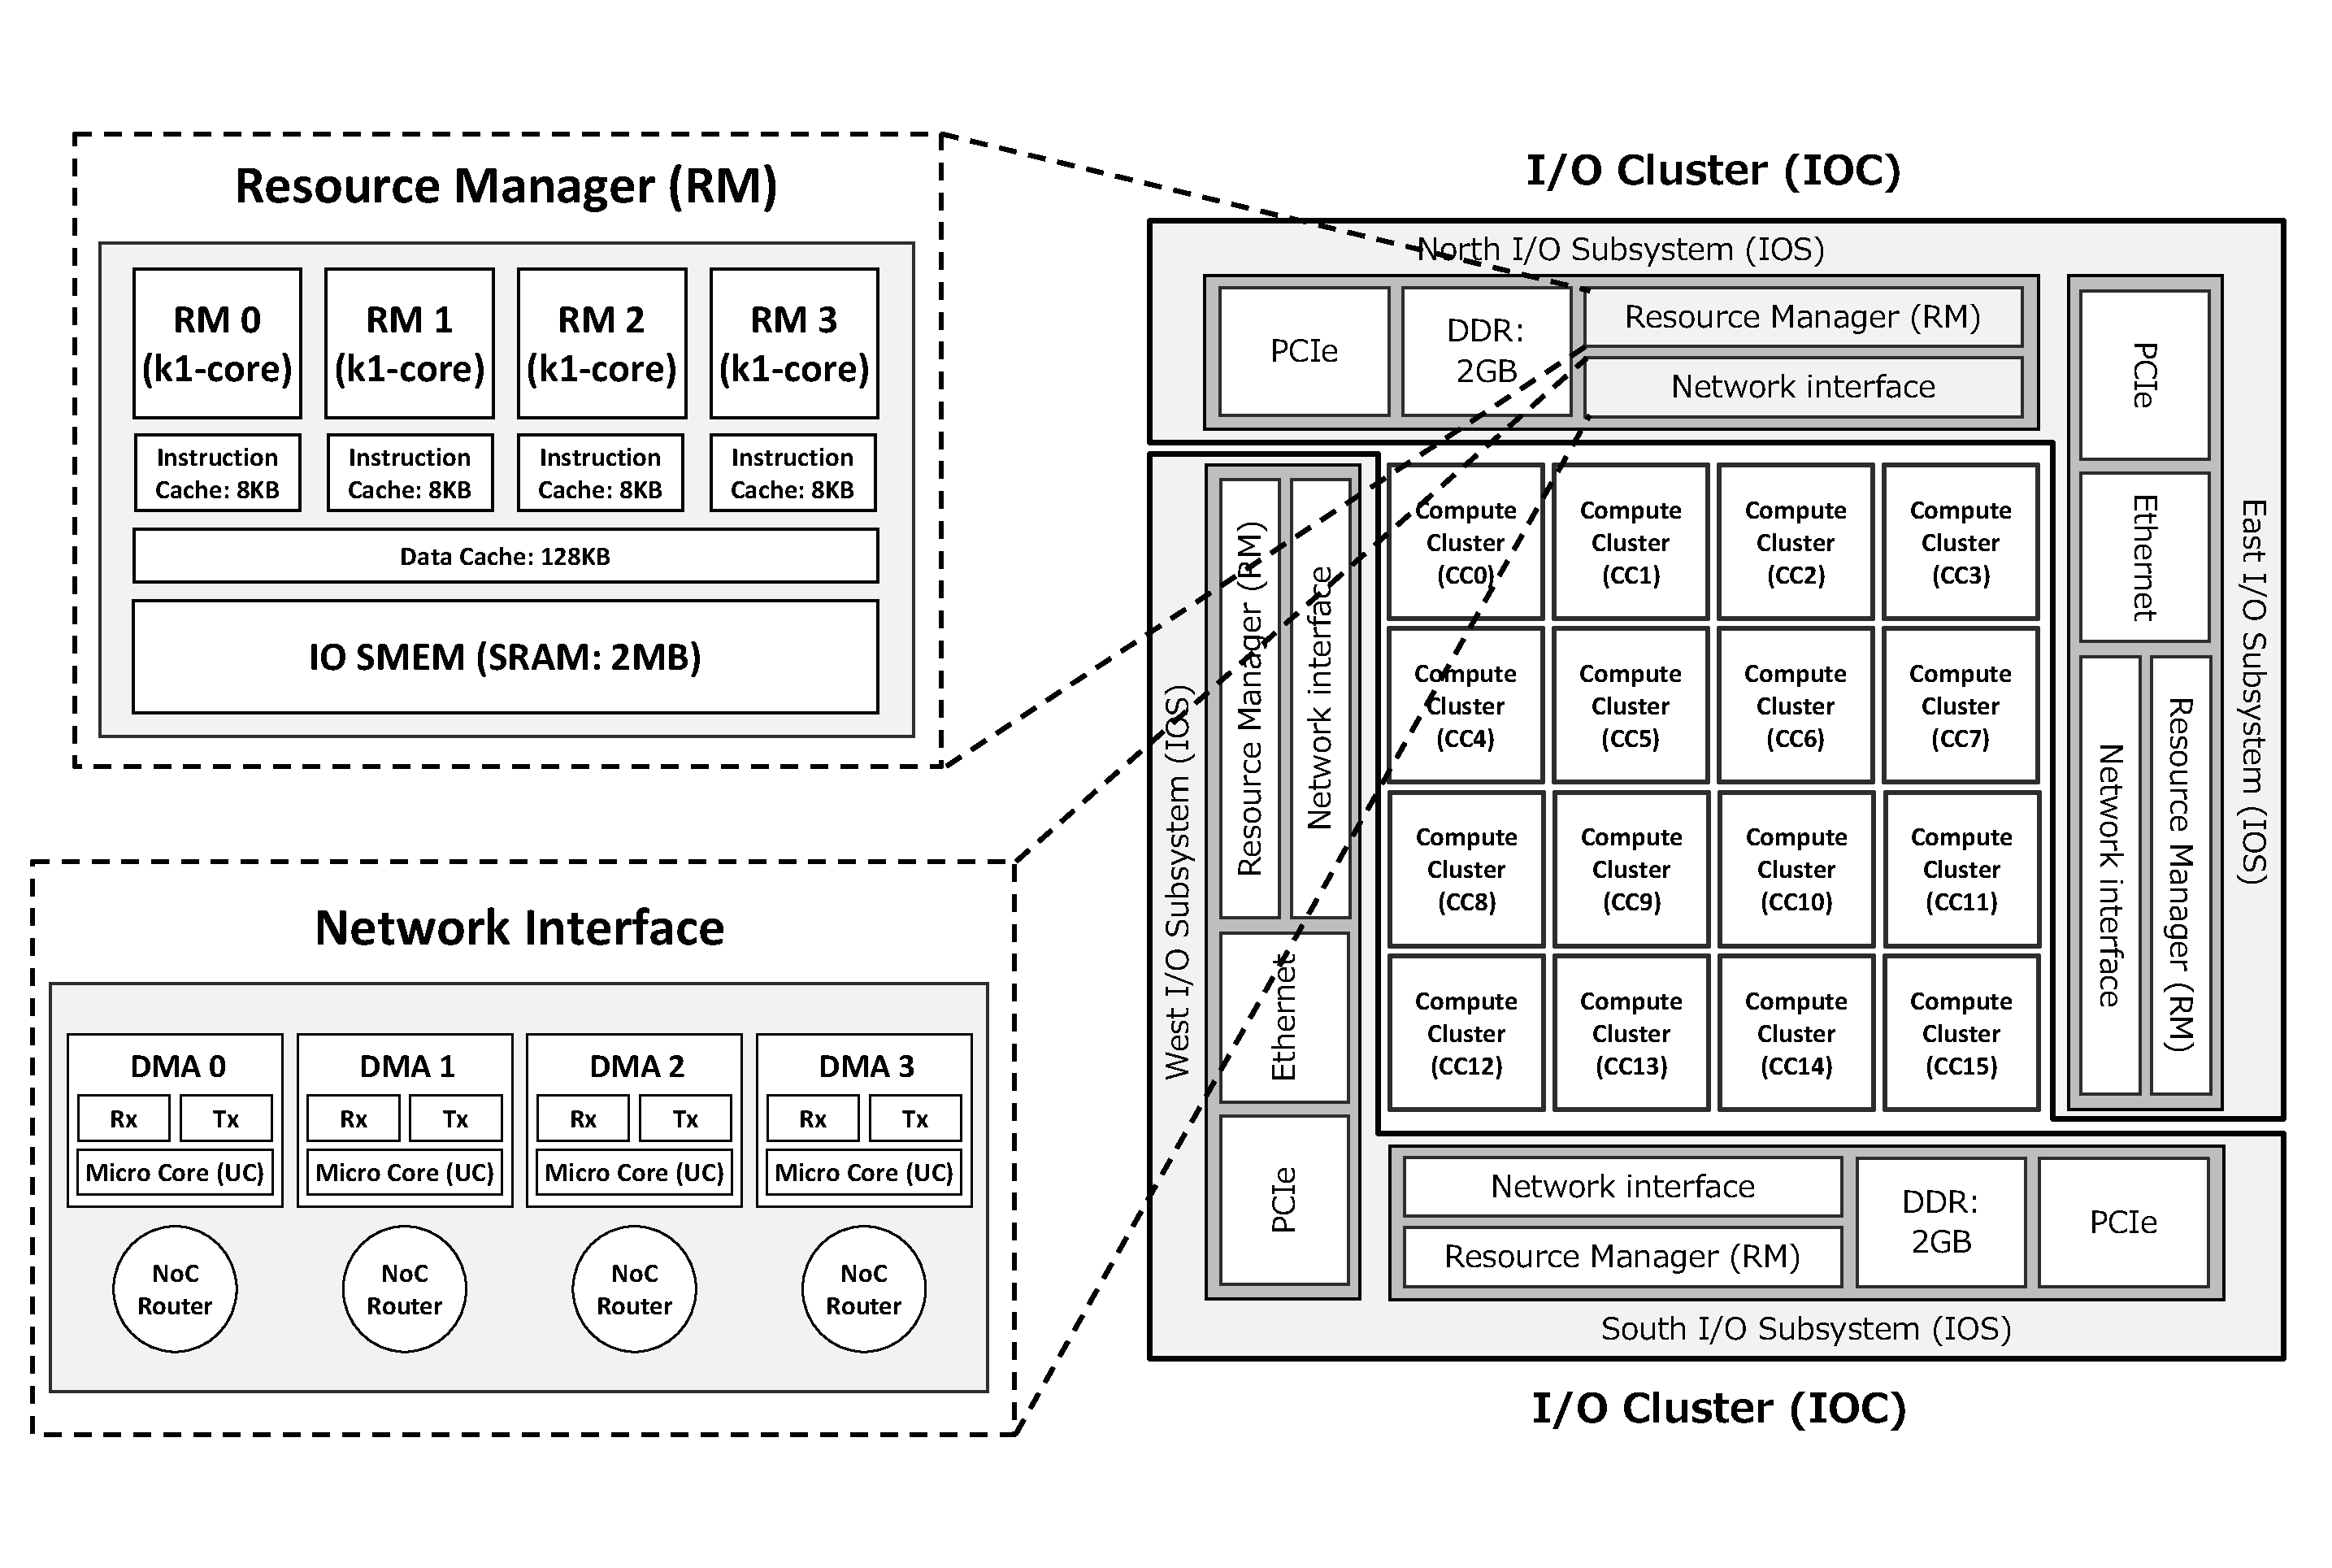
\includegraphics[width=1.0\linewidth]{../figure/mppa_architecture.eps}
  \caption{\label{fig:mppa_architecture}
    An overview of the architecture of the Kalray MPPA-256 Bostan.}
\end{figure}

\subsubsection{Compute Clusters (CC)}
\label{sec:cc}
In MPPA-256, the 16 inner nodes of the NoC correspond to the CCs.
Figure \ref{fig:cc_architecture} illustrates the architecture of each CC.

\begin{itemize}
\item \textbf{Processing Elements and an RM}:
In a CC, 16 processing elements (PEs) and a RM share 2 MB cluster local memory (SMEM) that is composed with 16 independent memory banks.
The capacity of each SMEM bank corresponds to 128 KB.
The PEs are mainly used by users for parallel processing.
Developers spawn computing threads on PEs.
The PEs and an RM in CC correspond to the Kalray-1 cores, which implement a 32-bit 5-issue Very Long Instruction Word architecture with 600 MHz (typical) or 800 MHz.
Each core is fitted with its own instruction and data caches.
Each cache is a 2-way associative with a capacity of 8 KB.
Thus, 17 k1-cores (a PE or the RM) share a multi-banked 2 MB SMEM.

\item \textbf{A Debug Support Unit (DSU) and a NoC Interface}:
In addition to PEs and an RM, bus masters on SMEM correspond to a DSU and a DMA engine in a NoC interface.
A DMA engine and a NoC router are laid out in a NoC interface.
In a manner similar to IOS, the CC DMA engine also has the following three interfaces: an Rx, a Tx, and a UC. 
It is instantiated in every cluster and connected to the SMEM.
\end{itemize}

\begin{figure}[t]
  \centering
  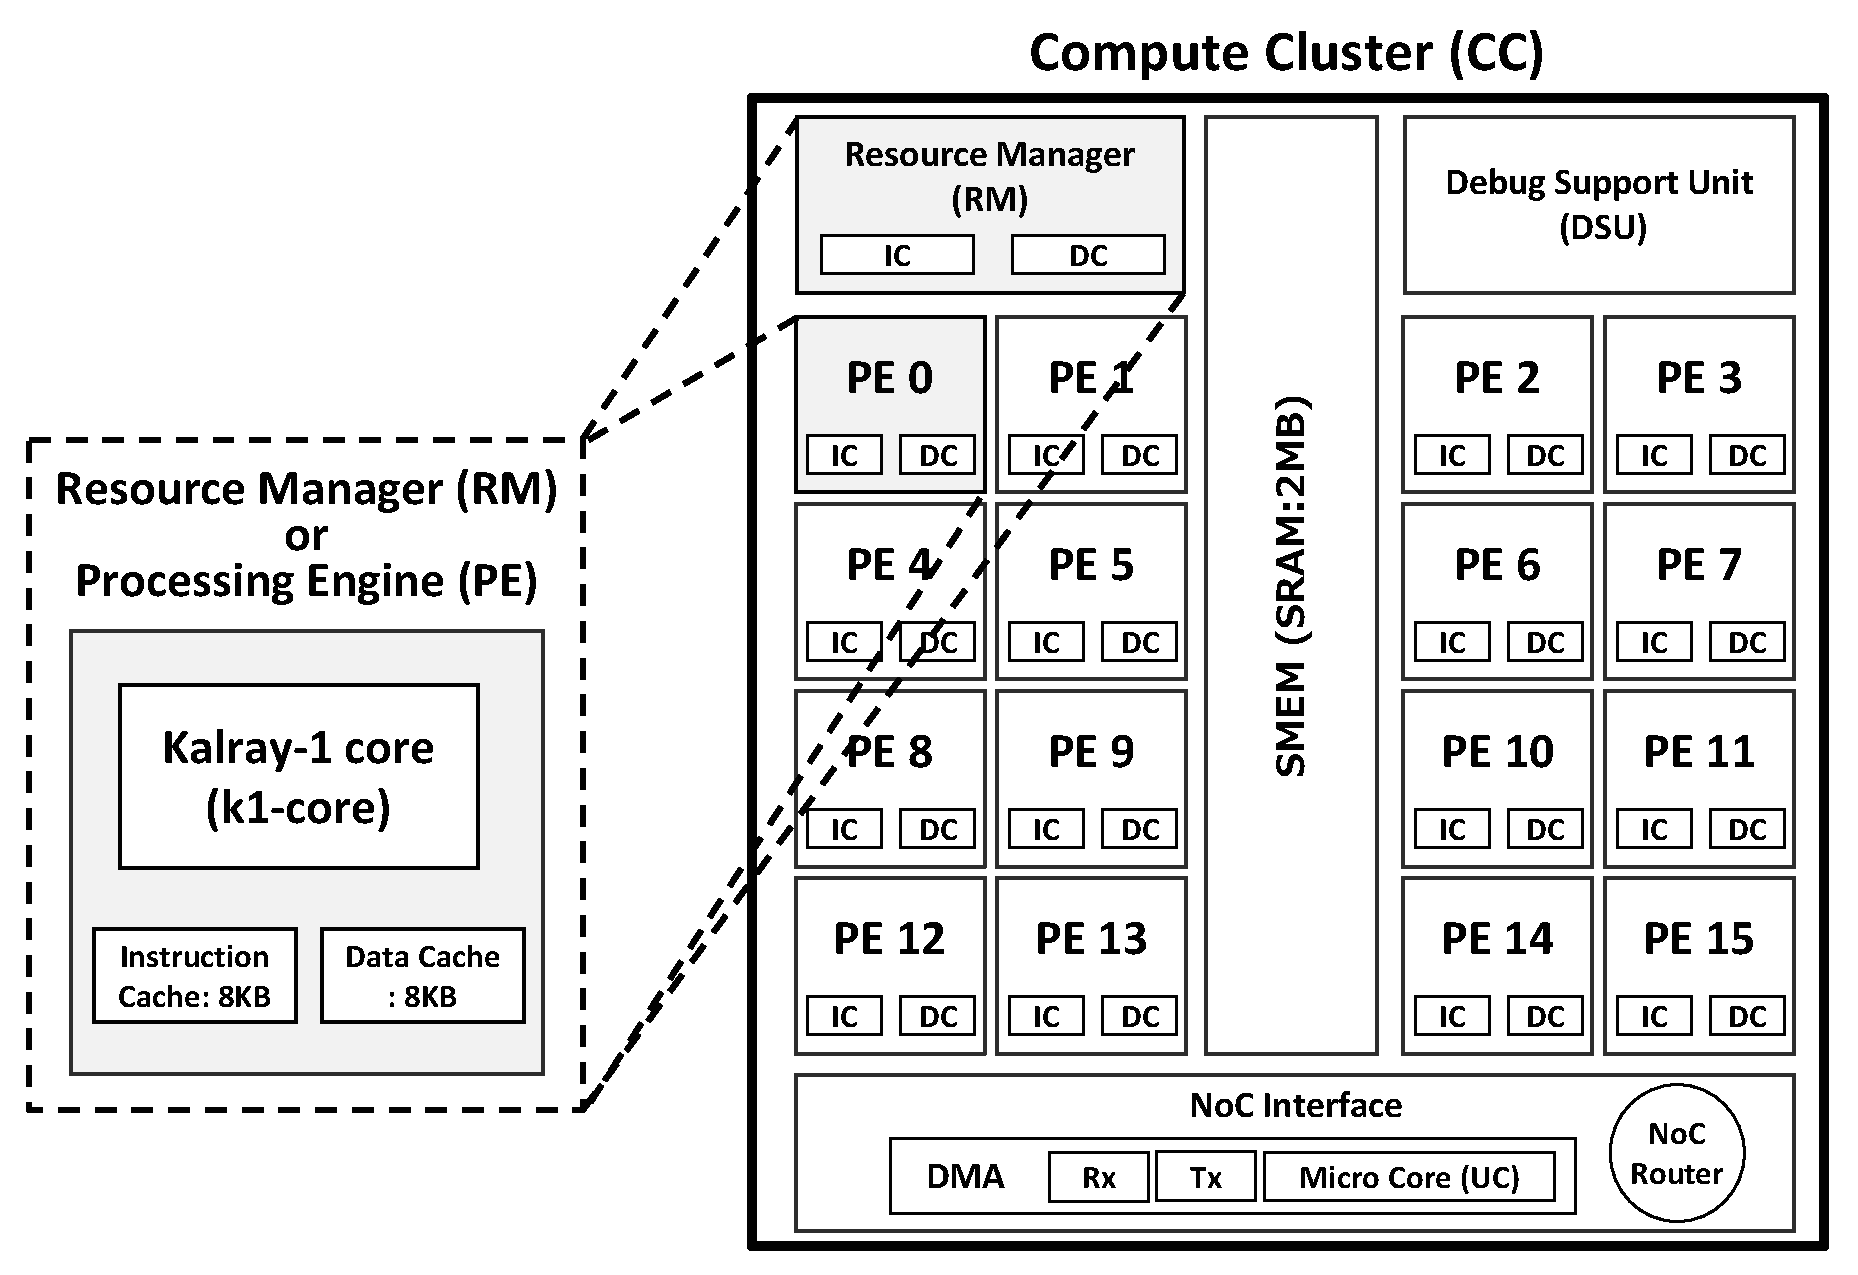
\includegraphics[width=1.0\linewidth]{../figure/cc_architecture.eps}
  \caption{\label{fig:cc_architecture}
    Compute Cluster architecture.}
\end{figure}


\subsubsection{Network-on-Chip (NoC)}
\label{sec:noc}
The 16 CCs and the 4 IOSs are connected by a NoC as shown in Figure \ref{fig:noc_map}.
Furthermore, a NoC is constructed on the bus network and has routers on each node.

\begin{itemize}
\item \textbf{Bus Network}:
Bus network connects nodes (CCs and IOSs) with torus topology \cite{dally2001route}
which has dual bands and involves a low average number of hops when compared to mesh topology \cite{vangal200780}, \cite{taylor2002raw}.
The network is actually composed of the following two parallel NoCs with bi-directional links (denoted by red lines in Figure \ref{fig:noc_map}):
the data NoC (D-NoC) that is optimized for bulk data transfers and the control NoC (C-NoC) that is optimized for small messages at low latency.
The NoC is implemented with wormhole switching and source routing.
Data are packaged in variable length packets that circulate between routers in a wormhole manner in which packets are broken into small pieces called flits (flow control digits).
The NoC traffic is segmented into packets, and each packet includes 1 to 4 header flits and 0 to 62 payload data flits.

\item \textbf{NoC routers}:
A node per compute cluster and four nodes per I/O subsystem holds the following two routers of its
own: a D-NoC router and a C-NoC router
Each RM or IO core on NoC node is associated with the fore-mentioned two NoC routers.
Furthermore, DMA engines in a NoC interface on the CC/IOS send and receive flits through the D-NoC routers with the Rx interface, the Tx interface, and the UC.
A mailbox component corresponds to the virtual interface for the C-NoC and enables one-to-one, N-to-one, or one-to-N low-latency synchronizations.
The NoC routers shown in Figures \ref{fig:mppa_architecture} and \ref{fig:cc_architecture} illustrate nodes as R0-15, R128-131, R160-163, R224-227, and R192-195 in Figure \ref{fig:noc_map}.
For purposes of simplicity, D-NoC/C-NoC routers are illustrated with a NoC router.
In both D-NoC and C-NoC, each network node (CC or IOS)  includes the following 5-link NoC routers:
four duplexed links for north/east/west and south neighbors and a duplexed link for local address space attached to the NoC router.
The NoC routers include FIFOs queuing flits for each direction.
The data links are four bytes wide in each direction and operate at the CPU clock rate of 600 MHz or 800 MHz, and therefore each tile can transmit/receive a total of 2.4 GB/s or 3.2 GB/s, which is spread across the four directions (i.e., north, south, east, and west).
\end{itemize}

\begin{figure}[t]
  \centering
  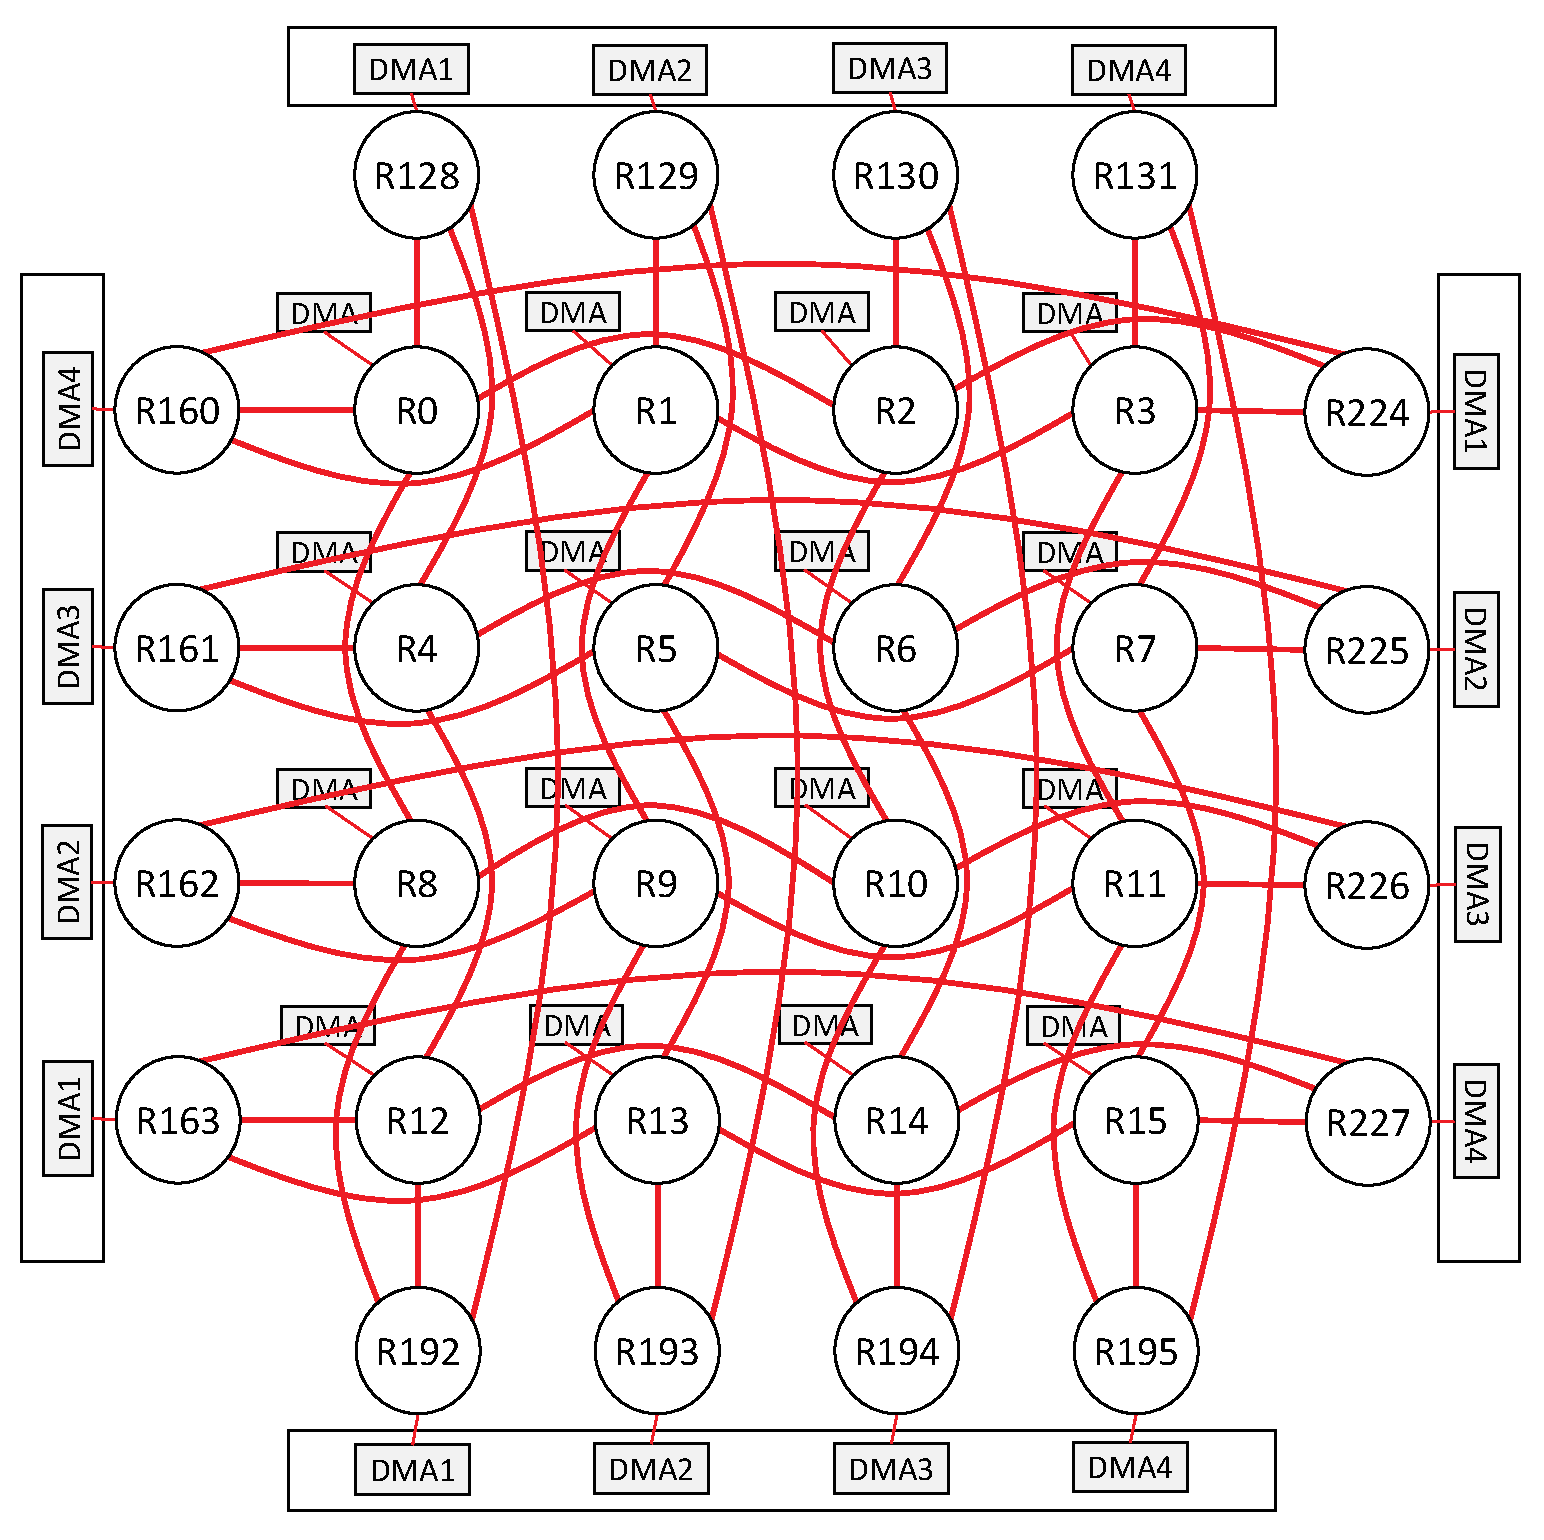
\includegraphics[width=1.0\linewidth]{../figure/noc_map.eps}
  \caption{\label{fig:noc_map}
    NoC connections (both D-NoC and C-NoC).}
\end{figure}

\subsection{Software Model}
\label{sec:software_model}
Figure \ref{fig:software_stack} shows the software stack used for Kalray MPPA-245 in the present study.
The Kalray system is an extensible and scalable array of computing cores and memory.
With respect to this type of a system, it is possible to map several programing models or runtimes such Linux, real-time operating system, POSIX API, OpenCL, and OpenMP.
Each layer is described in detail.

In the hardware abstraction layer, an abstraction package abstracts hardware of a CC, IOS, and NoC.
The abstraction package serves as a system that does not provide any services.
The hardware abstraction is responsible for partitioning hardware resources and controlling access to the resources from the user-space operating system libraries.
Additionally, the abstraction package retrieves resources allocated to a partition at any time.
It sets-up and controls inter-partition communications as a virtual machine abstraction layer.
The hardware abstraction runs on the dedicated RM core.
All the services are commonly provided by a rich operating system (for e.g., virtual memory, interrupts, and schedule) that must be provided by user-space libraries.
Consequently, each runtime or operating system implements its own services that are optimized to specific needs.
This is because each programing model or runtime involves different requirements.
A minimal kernel avoids wastage of resources and mismatched needs.

In a low-level library layer, the Kalray system also provides libraries for handling NoC.
Additionally, NoC features such as routing and quality of service are set by the programmer.
The Libnoc allows direct access to memory mapped registers for their configurations and uses.
It is designed to cause a minimum amount of CPU overhead.
It also serves as a minimal abstraction for resource allocation.
Librouting offers a minimal set of functions that can be used to route data between any clusters of the MPPA including unicast (one target) modes or multicast (multiple targets) modes.
As shown in Figure \ref{fig:noc_map}, routing on the torus network is statically conducted with its own policy.
The Libpower enables spawning and waiting for the end of execution of a remote cluster.

Various operating systems support the abstraction package in the OS layer.
The following Real-Time Operating System (RTOS) is introduced:
\begin{itemize}
\item \textbf{RTEMS}: RTEMS (Real-Time Executive for Multiprocessor Systems) is a full featured RTOS prepared for embedded platforms.
It supports several APIs and standards, and most notably supports the POSIX API.
The system provides a rich set of features, and an RTEMS application mostly corresponds to a regular C or C++ program that uses the POSIX API.
Additionally, RTEMS can be built on the IOC.
\item \textbf{NodeOS}: On CC, the MPPA cluster operating system utilizes a runtime called NodeOS.
The OS addresses the need for a multicore OS to conform to the maximum possible extent to the standard POSIX API.
The NodeOS enables a user code by using POSIX API to run on PEs on CC.
First, NodeOS runtime starts on PE0 prior to before calling the user main function.
Subsequently, \texttt{pthread} is called on other PEs.
\item \textbf{eMCOS}: On both CC and IOS, eMCOS provides minimal programing interfaces and libraries.
Specifically, eMCOS is a real-time embedded operating system developed by eSOL (a Japanese supplier for RTOS), and eMCOS is the world's first commercially available many-core RTOS for use in embedded systems.
The OS implements a distributed micro-kernel architecture.
This compact micro-kernel is equipped with only minimal functions.
It enables applications to operate priority based message passing, local thread scheduling, and thread management on IOS as well as CC.
\end{itemize}
RTMES and NodeOS are provided by Kalray and eMCOS is released by eSOL.

\begin{figure}[t]
  \centering
  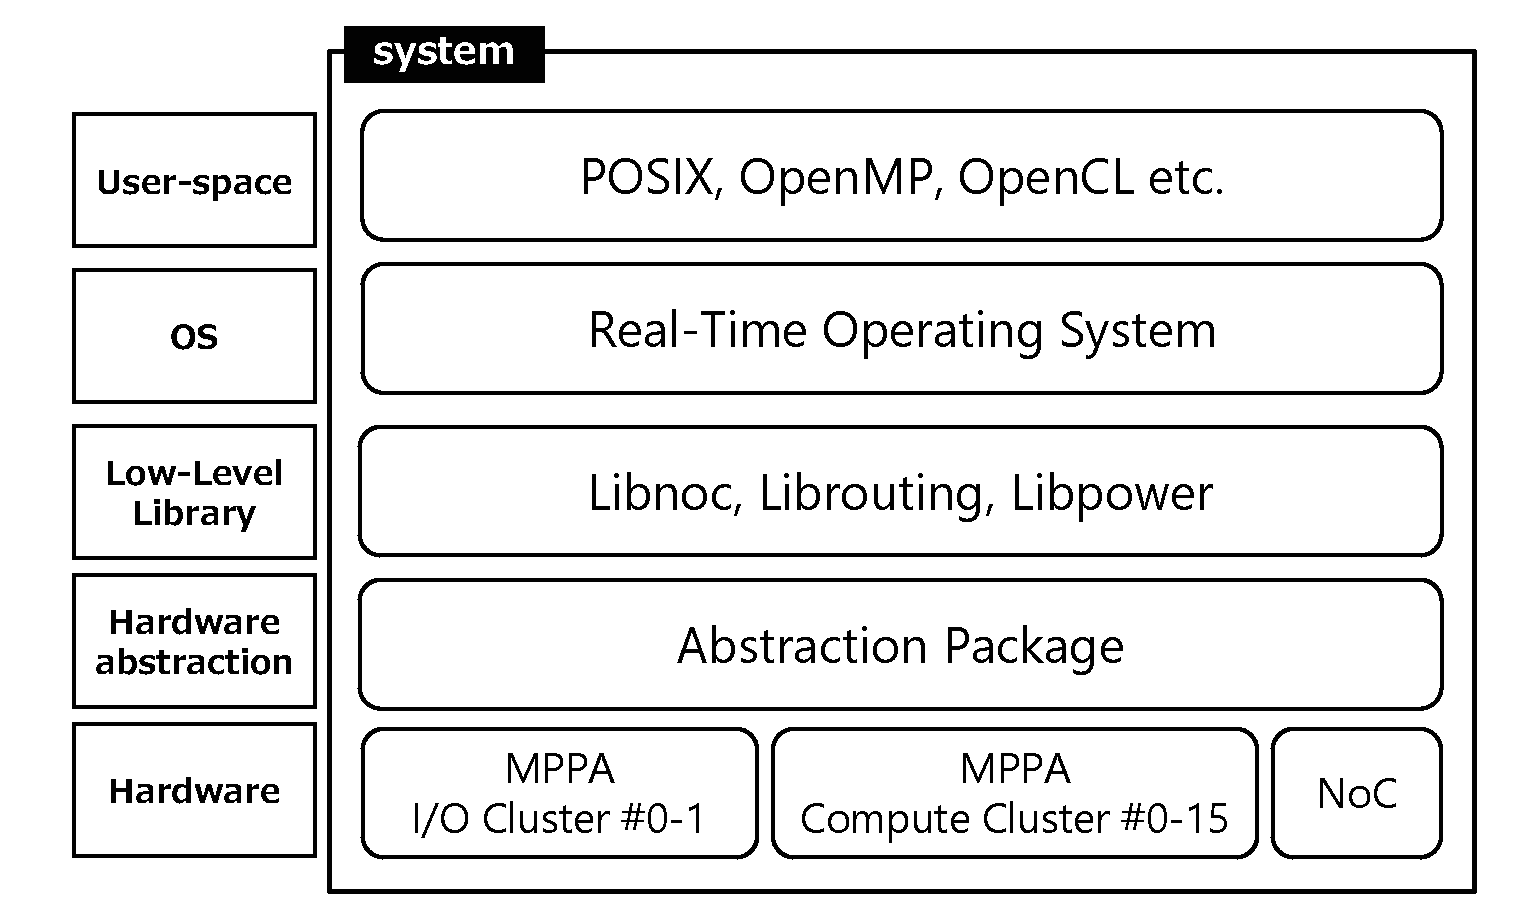
\includegraphics[width=1.0\linewidth]{../figure/softwarestack.eps}
  \caption{\label{fig:software_stack}
    The software stack of Kalray MPPA-256.}
\end{figure}


\section{Data Transfer Framework}
\label{sec:framework}
In this section, data transfer methods in MPPA-256 are explained.
For scalability purposes, MPPA-256 accepts clustered architectures in which each cluster contains its own memory.
16 cores are packed as a cluster and they share 2 MB memory (SMEM) as shown in Figure \ref{fig:cc_architecture}.
This avoids frequent memory contention due to numerous cores and helps in increasing the number of cores.
However, the architecture constraints memory sthat can be directly accessed by the cores.
In order to communicate with cores outside the cluster, it is necessary to transfer data between clusters through the D-NoC with NoC interfaces.

A Rx interface exists in the receiving side to receive data with DMA.
It is necessary to allocate a D-NoC Rx resource and configure it to wait to receive the data.
A DMA in a NoC interface contains 256 D-NoC Rx resources.
Two interfaces, namely a Tx interface and a UC interface as explained in Sections \ref{sec:ios} and \ref{sec:cc},
are present with respect to the sending side for users to send data between clusters.
The UC is a network processor that is programmed to set threads to send data in DMA.
It executes programed pattern and sends data through the D-NoC without a PE and an RM.
The UC interface results in higher data transfer throughput compared to the direct activation of the Tx interface by a RM or PE core.
However, a DMA in a NoC interface contains only 8 D-NoC UC resources.
Both interfaces use a DMA engine to access memory and copy data.
Irrespective of whether or not a UC interface is used, it is necessary to allocate a D-NoC Tx resource and configure it to send data.
Additionally, it is necessary to allocate and configure D-NoC UC resources if a UC interface is used.

% We list following two data transmit patterns.
% \begin{itemize}
% \item \textbf{Tx+PE}: 
% \item \textbf{Tx+UC}:
% \end{itemize}

\section{Evaluations}
\label{sec:evaluations}
This section involves examining two types of evaluations, namely a D-NoC data transfer evaluation in which latency characteristics of interfaces and memory type are explored and a matrix calculation evaluation that demonstrates the parallelization potential of the MPPA-256 and its memory access characteristics while dealing with large data.

\subsection{D-NoC Data Transfer}
\label{sec:dnoc_eval}
This evaluation involves clarifying end-to-end latency by considering the relation among interfaces (Tx or UC), routing on NoC, and memory type (DDR or SMEM).
This is achieved by preparing four routes as shown in Figure \ref{fig:noc_routes}.
The routes on D-NoC map (Figure \ref{fig:noc_map}) contains various connections between routers, namely a direct link, a cross link, and a flying link.
With respect to case of routes from the IOS routers to the CC routers, transmitted data is allocated in DDR or IO SMEM.
The CC only includes SMEM as shown in Figure \ref{fig:cc_architecture}.
A low-level library is directly used to transfer data with D-NoC.
The transferred data correspond to 100 B, 1 KB, 10 KB, 100 KB, and 1 MB.
The buffers are sequentially allocated in DDR or SRAM (IO SMEM or CC SMEM).
The capacity of CC SMEM corresponds to 2 MB, and thus it is assumed that the appropriate communication buffer size corresponds to 1 MB.
Given the assumption, the other memory area corresponds to the application, library, and operating system.
End-to-end latencies are measured 1,000 times in numerous situations as shown in Figures \ref{fig:DDR_tx}, \ref{fig:DDR_uc}, \ref{fig:IO_SMEM_tx}, and boxplots are obtained as depicted in Figures \ref{fig:IO_SMEM_uc}, \ref{fig:tx_uc_log} and \ref{fig:tx_uc}.
The following evaluations are conducted on eMCOS.

\begin{figure}[t]
  \centering
  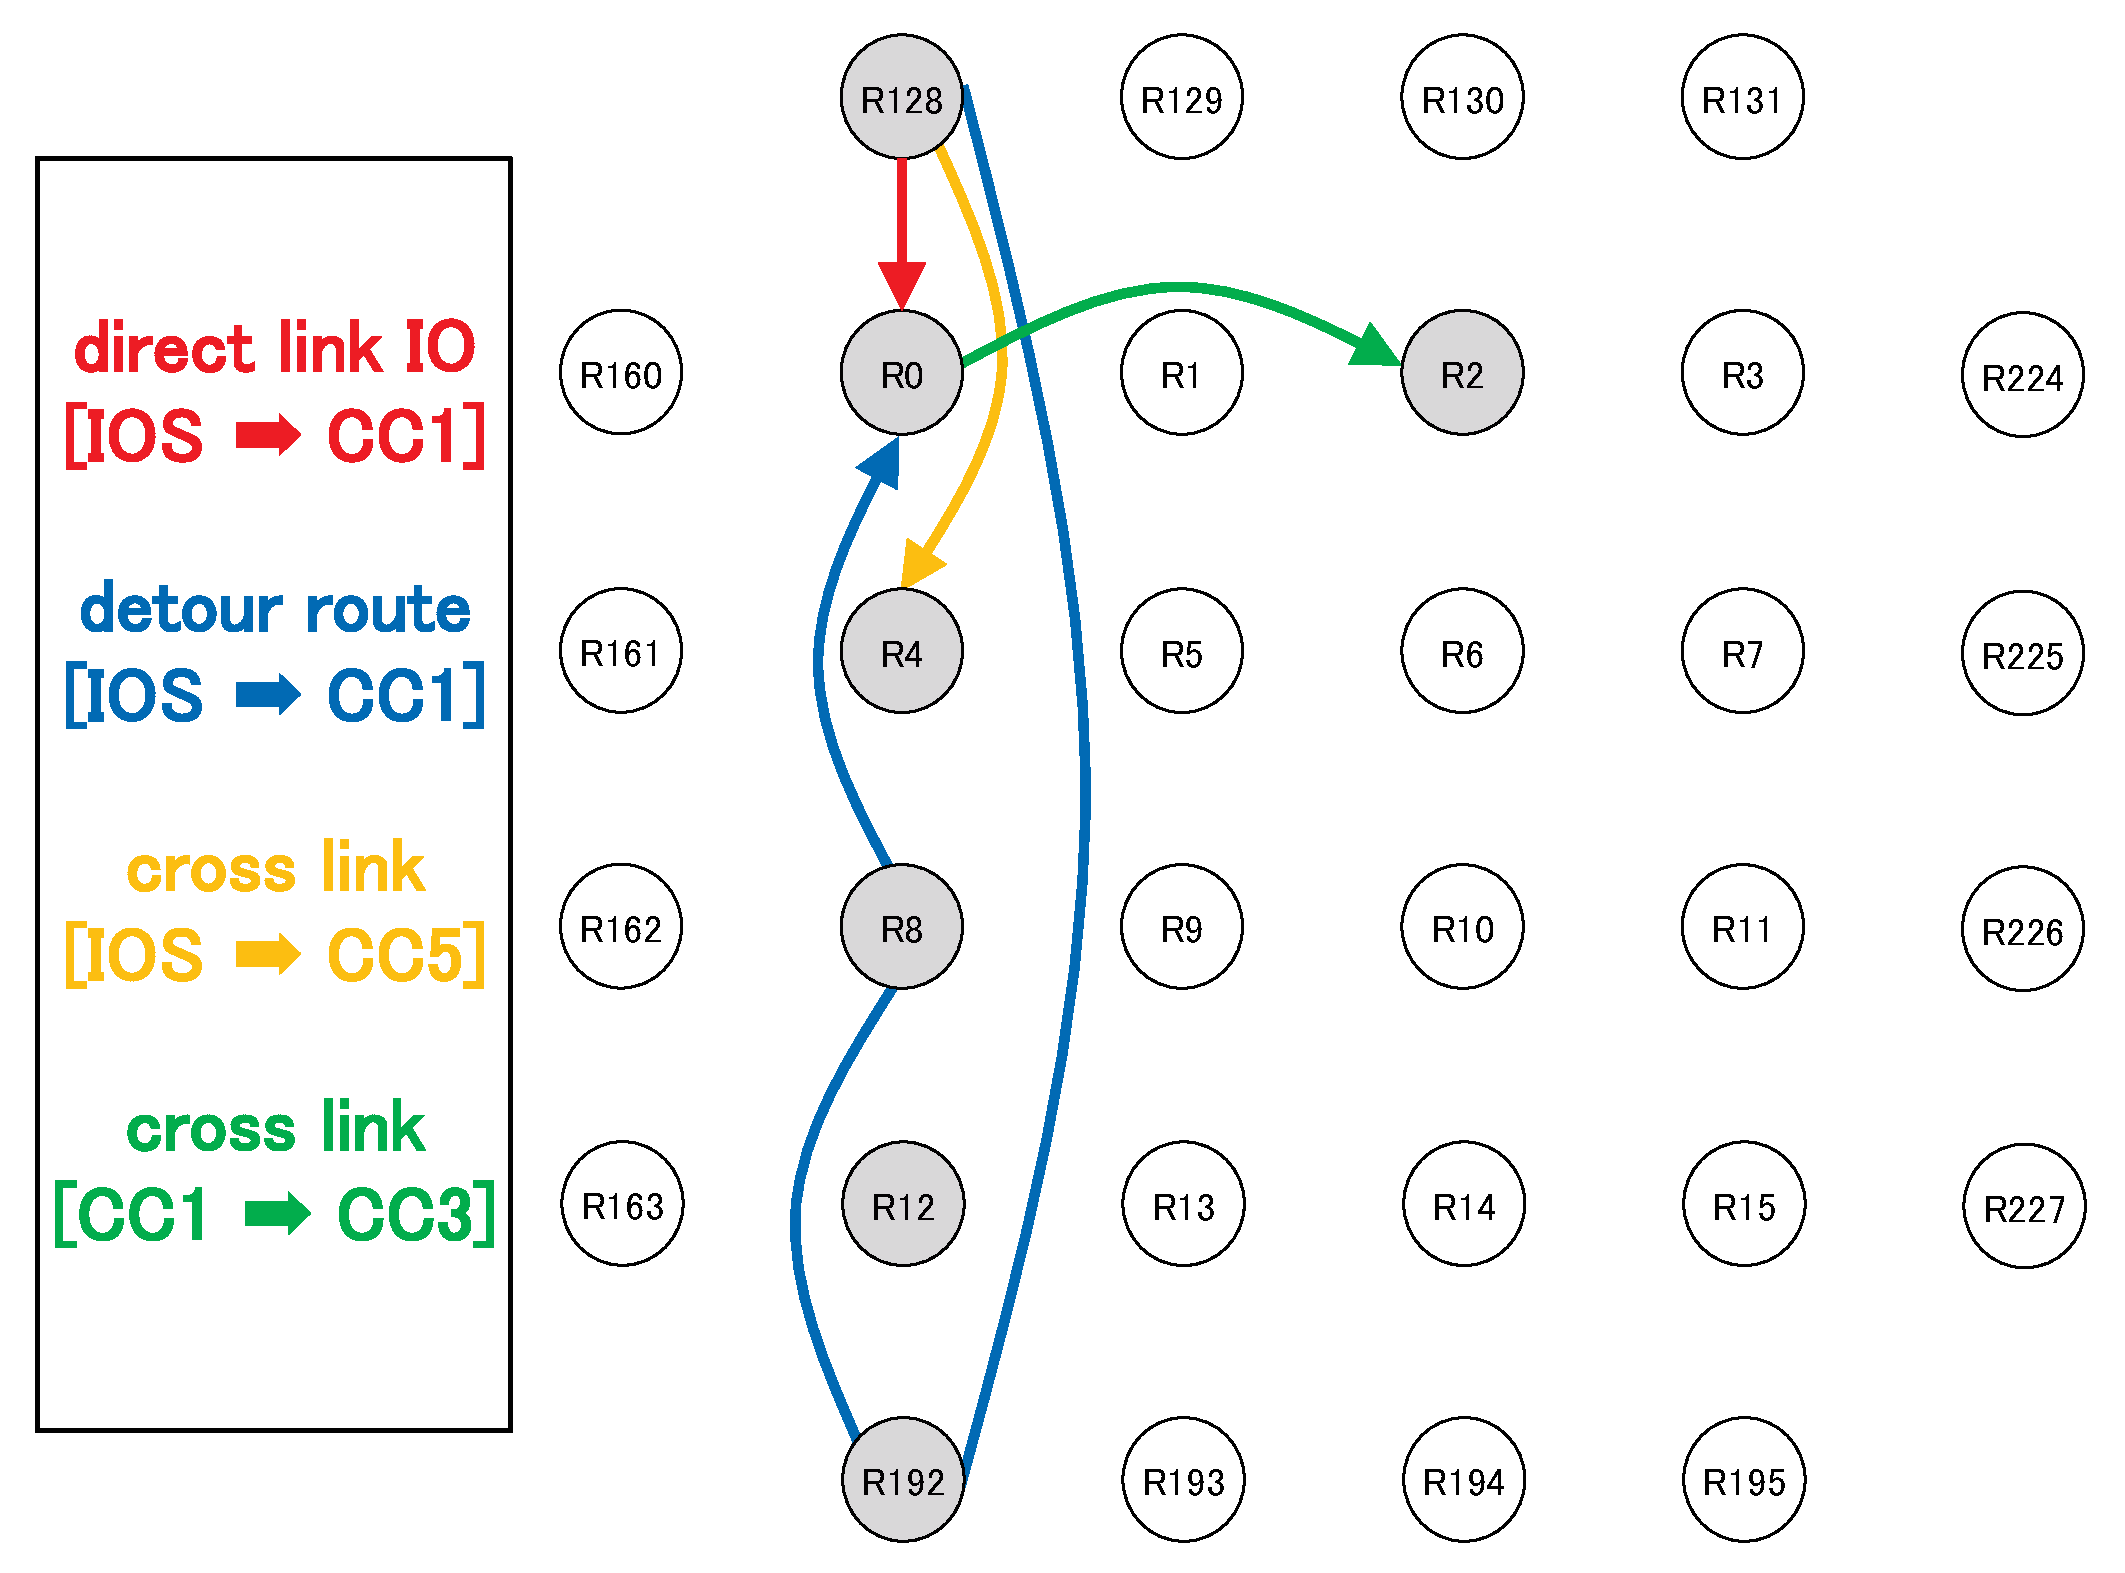
\includegraphics[width=1.0\linewidth]{../figure/noc_routes.eps}
  \caption{\label{fig:noc_routes}
    Four D-NoC routes used in the evaluation.}
\end{figure}

Data transfer latencies between IOS and CC are not influenced by routing.
This involved preparing two interfaces (Tx and UC), three routes(direct link, cross link, and detour route), and two memory locations in which the transferred data is allocated.
As shown in Figures \ref{fig:DDR_tx}, \ref{fig:DDR_uc}, \ref{fig:IO_SMEM_tx}, and \ref{fig:IO_SMEM_uc}, 
end-to-end latency scales exhibit a linear relation with data size, and there are no significant differences between the three routes with respect to data transfer latency.
This result is important in torus topology NoC because the number of minimum steps exceeds those in the mesh topology. 
It is observed that queuing in the NoC routers and hardware distance on the NoC are not dominant factors for latency.
The time taken by transmitting and receiving transactions exceeds those of other transaction.
Additionally, it is briefly recognized that the speed of UC exceeds that of Tx.
The data is arranged as shown in Figures \ref{fig:tx_uc_log} and \ref{fig:tx_uc} to facilitate a precise analysis with
respect to the interface and memory location.
In the figures, only the cross link from IOS to CC5 is accepted because routes do not influence latency.
In order to facilitate intuitive recognition, two kinds of figures are arranged, namely a logarithmic axis and a linear axis.

\begin{figure*}[t]
  \tabcolsep = 0.5mm              % side-margin in column
  \begin{tabular}{cccc}
    \begin{minipage}[t]{0.24\textwidth}
      \includegraphics[width=1.0\linewidth]{../../R/mppa/graph/eps/BoxPlot_DDR_tx.eps}
      \vspace{-7mm}
      \caption{Data transfer with Tx from IO DDR to CC.}
      \label{fig:DDR_tx}
    \end{minipage}
    &
    % \setcounter{figure}{8}
    \begin{minipage}[t]{0.24\textwidth}
      \includegraphics[width=1.0\linewidth]{../../R/mppa/graph/eps/BoxPlot_DDR_uc.eps}
      \vspace{-7mm}
      \caption{Data transfer with UC from IO DDR to CC.}
      \label{fig:DDR_uc}
    \end{minipage}
    &
    % \setcounter{figure}{10}
    \begin{minipage}[t]{0.24\textwidth}
      \includegraphics[width=1.0\linewidth]{../../R/mppa/graph/eps/BoxPlot_IO_SMEM_tx.eps}
      \vspace{-7mm}
      \caption{Data transfer with Tx from IO SMEM to CC.}
      \label{fig:IO_SMEM_tx}
    \end{minipage}
    &
    % \setcounter{figure}{7}
    \begin{minipage}[t]{0.24\textwidth}
      \includegraphics[width=1.0\linewidth]{../../R/mppa/graph/eps/BoxPlot_IO_SMEM_uc.eps}
      \vspace{-7mm}
      \caption{Data transfer with UC from IO SMEM to CC.}
      \label{fig:IO_SMEM_uc}
    \end{minipage}
    \vspace{-3mm}
  \end{tabular}
  \vspace{+3mm}
\end{figure*}

In the Tx interface, DDR causes a large increase in latency.
The time taken by the DDR is twice as that of the IO SMEM as shown in Figure \ref{fig:tx_uc}.
This is due to the memory access speed characteristics of DRAM and SRAM.
In the case of the Tx interface, it is necessary for an IO core on IOS to operate the DMA in the IOS NoC interface.
This is attributed to the fact that the core is involved in processing.
The speed of the data transfer latency between CCs exceeds that between IOS and CC.
This result indicates that the MPPA-256 is optimized for communication between the CCs.

With respect to the UC interface, the latency is not significantly affected by the location at which the transferred buffer is allocated (i.e., the DDR or SMEM).
Similar latency characteristics are observed in Figures \ref{fig:tx_uc_log} and \ref{fig:tx_uc}.
In the case of the UC interface, an IO core on the IOS does not involve a DMA transaction.
A micro core in the NoC interface executes a programed thread sending data.
This evaluation result suggests that the slow access speed of the DDR is not significant in the case of the UC.
In a manner similar to the Tx interface, the speed of the data transfer latency between CCs exceeds that between IOS and CC.

\begin{figure*}[t]
  \tabcolsep = 0.5mm              % side-margin in column
  \begin{tabular}{cc}
    % \setcounter{figure}{9}
    \begin{minipage}[t]{0.49\textwidth}
      \includegraphics[width=1.0\linewidth]{../../R/mppa/graph/eps/BoxPlot_Tx_vs_UC_log.eps}
      \vspace{-7mm}
      \caption{Data transfer with Tx/UC (logarithmic axis).}
      \label{fig:tx_uc_log}
    \end{minipage}
    &
    % \setcounter{figure}{11}
    \begin{minipage}[t]{0.49\textwidth}
      \includegraphics[width=1.0\linewidth]{../../R/mppa/graph/eps/BoxPlot_Tx_vs_UC.eps}
      \vspace{-7mm}
      \caption{Data transfer with Tx/UC (linear axis).}
      \label{fig:tx_uc}
    \end{minipage}
    \vspace{-3mm}
  \end{tabular}
  \vspace{+2mm}
\end{figure*}


\subsection{Matrix Calculation}
\label{sec:martix_eval}

\subsubsection{Situations and Assumptions}
\label{sec:situations_and_assumptions}
In the evaluation, matrix calculation time and parallelization potential of MPPA-256 are clarified.
Matrix calculations are conducted in IOS and CC.
Three computing situations are considered as shown in Figure \ref{fig:mat_calc}.
The first situation involves computing in IOS where four cores are available.
In order to analyze memory access characteristics, a matrix buffer is allocated in IO DDR and SMEM.
The second situation involves computing in CC in which 16 cores are available.
The third situation involves offload-computing by using an IOS and four CCs.
Parallelized processing is executed with four CCs' cores and SMEMs.
A few cores in IOS and CC manage the parallelized transaction.
The method can handle large data in which one cluster is not
sufficient because buffer capacity is not limited to 2MB in SMEM.
Parallelized processing and the total capacity of SMEM are superior to IOS or CC computations. 
With respect to the IOS, the application can handle large capacity data only in the DDR.
However, in this method, distributed memories are used to deal with large capacity data in SMEM.
Thus, it is necessary for IOS and CC cores to access matrix buffers without cache to avoid cache coherency trouble.
In order to facilitate faster data transfer, a part of the matrix buffer is transmitted in parallel as shown in Figure \ref{fig:mat_calc}.

Matrix calculation time is analyzed with parallelization and memory allocation.
Additionally, the influence of cache is analyzed because cache coherency is an important issue in many-core system.
There are several cases in which applications must access specific memory space without a cache.
With respect to the given assumptions, maximum total buffer size corresponds to 1 MB, and thus three matrices buffers are prepared, and each size corresponds to 314 KB.
Matrix A and matrix B are multiplied, and the result is stored in matrix C.
The total of the three matrices is set as approximately 1 MB.
In CC, we assume that the remainder of SMEM (1 MB) is occupied with system software and applications.
The following evaluations are conducted on eMCOS.

\begin{figure}[t]
  \centering
  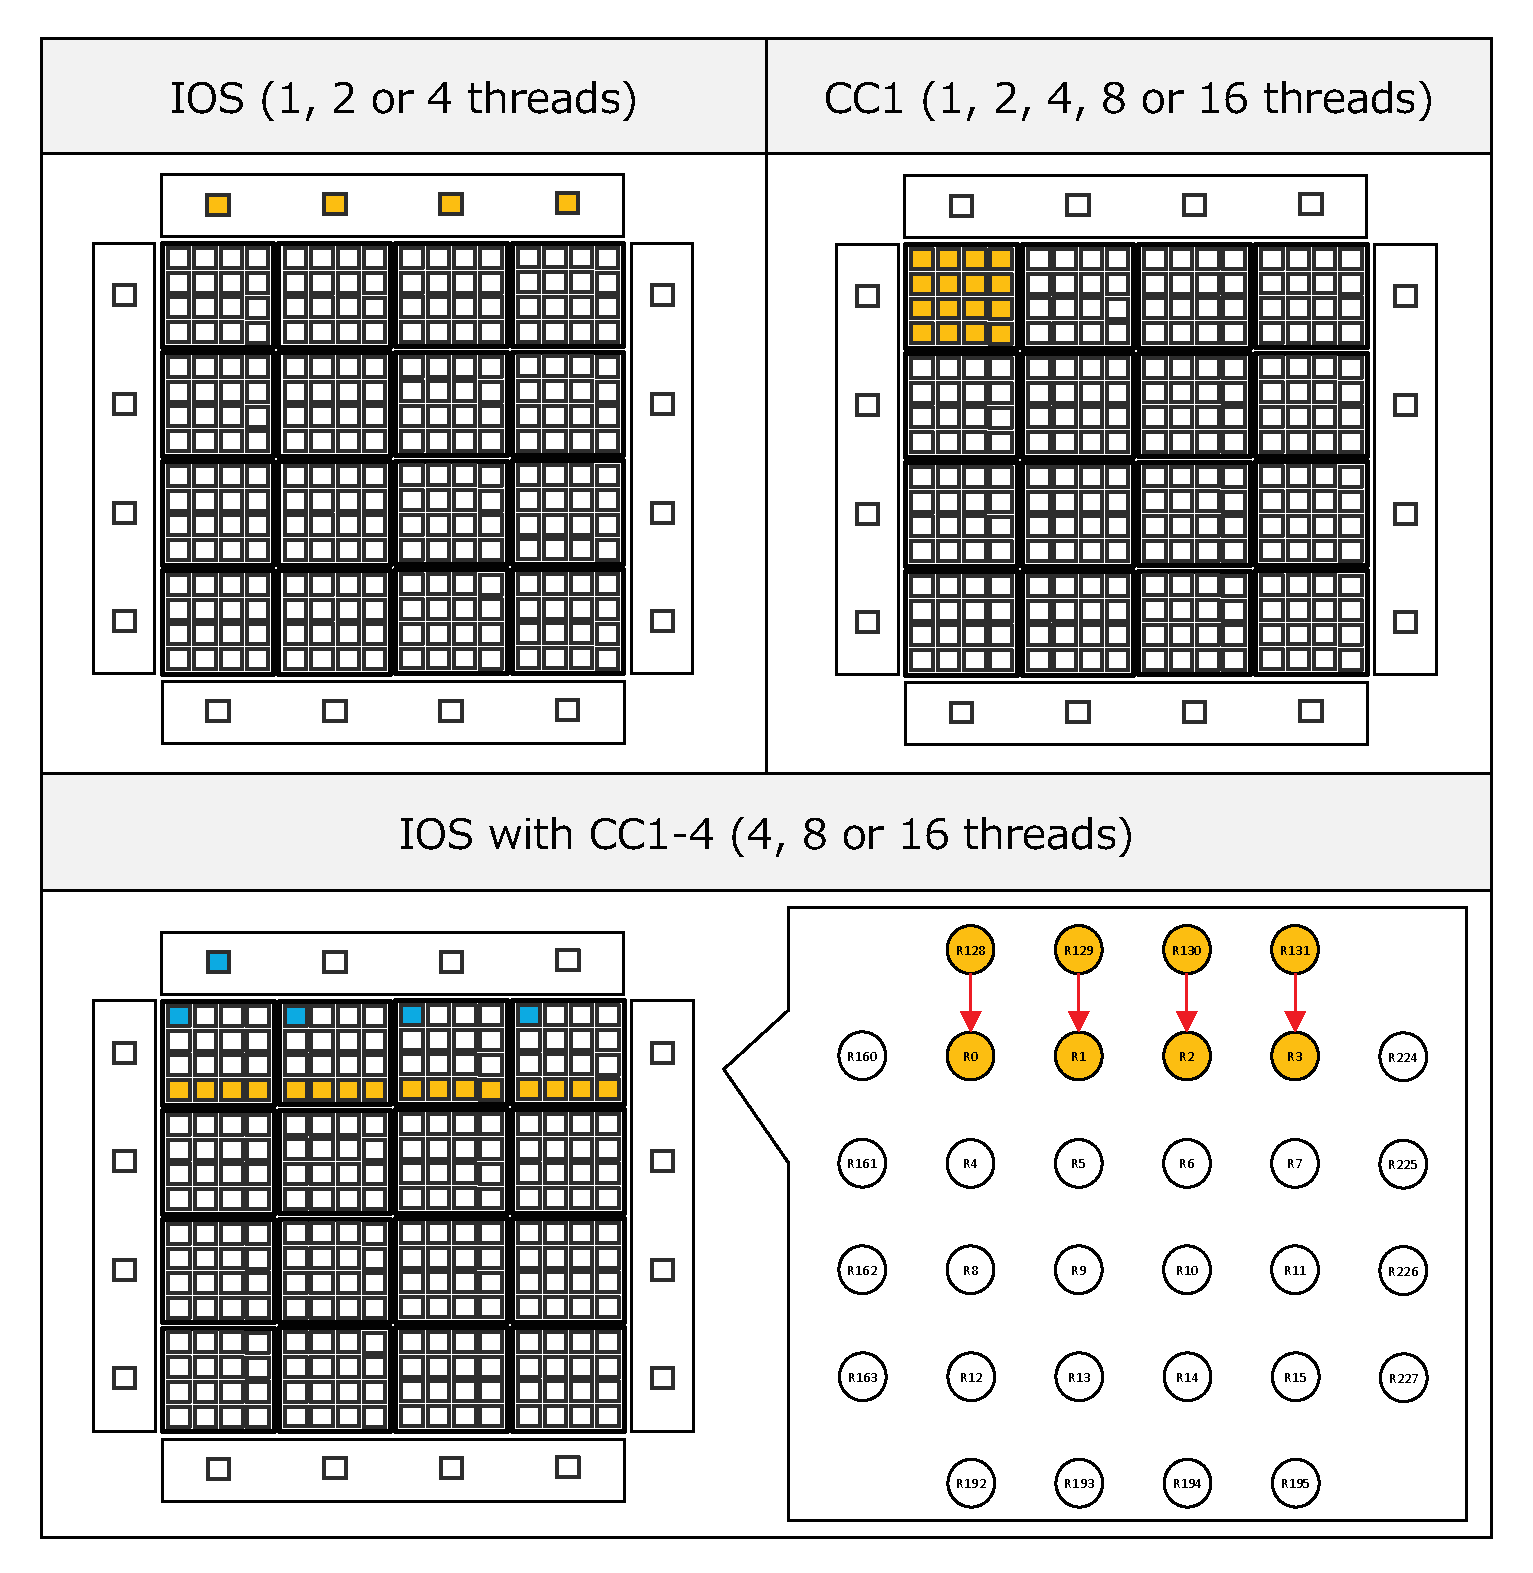
\includegraphics[width=1.0\linewidth]{../figure/matrix_calculation.eps}
  \caption{\label{fig:mat_calc}
    Matrix calculation situations.}
\end{figure}

\subsubsection{Influence of Cache and Memory}
\label{sec:cache_and_memory}
First, matrix calculation time with the cache in IOS and CC is depicted in Figure \ref{fig:mat_calc_cash}.
There are almost no differences between IO DDR, IO SMEM, and CC SMEM due to the cache.
Furthermore, 128 KB data cache in the IOS works well and compensates for the DDR delay.
Additionally, it is observed that calculation time scales exhibit a linear relation with the number of threads.
This corresponds to ideal behavior with respect to parallelization.

Second, matrix calculation time without cache in the IOS and CC is shown in Figure \ref{fig:mat_calc_uncash}.
The absence of a cache, results in a fourfold increase in the DDR and a high difference arises with respect to the SMEM.
Another notable result is that calculation speed in CC SMEM exceeds that of the IO SMEM.
This characteristic is hidden in the calculation with the cache.
The computing cores involve the same k1-cores in IOS and CC, and thus it is considered that the characteristics and physical arrangement of SMEM exert a significant effect.
This is an interesting result since a high difference that cannot be ignored exists.
It is also observed that calculation time exhibits a linear relation with the number of threads.
Furthermore, the calculation speed without the cache in CC SMEM exceeds that with cache.
This result is contrary to intuition, and the two factors are conceivable.
A small data cache (8 KB) in CC does not function adequately and direct assembly instruction for uncached access optimizes memory access.

\begin{figure*}[t]
  \tabcolsep = 0.5mm              % side-margin in column
  \begin{tabular}{cc}
    \begin{minipage}[t]{0.49\textwidth}
    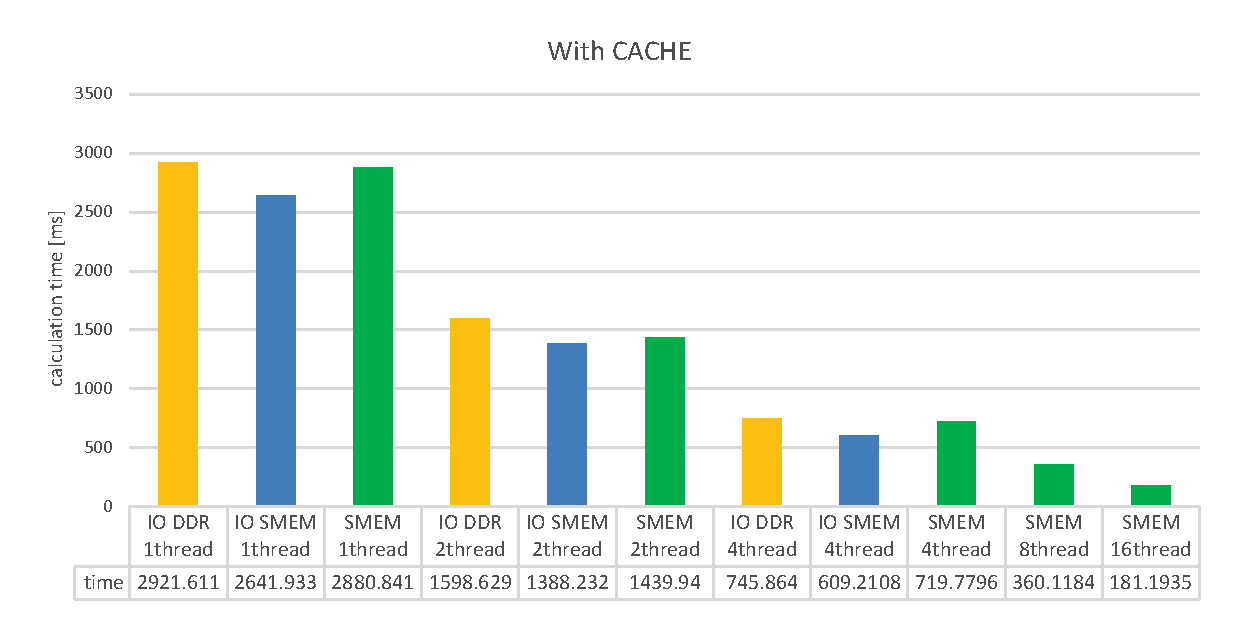
\includegraphics[width=1.0\linewidth]{../figure/BarGraph_matrix_with_cache.eps}
      % \vspace{-7mm}
      \caption{Matrix calculations in IOS and CC with cache.}
      \label{fig:mat_calc_cash}
    \end{minipage}   
    &
    % \setcounter{figure}{11}
    \begin{minipage}[t]{0.49\textwidth}
      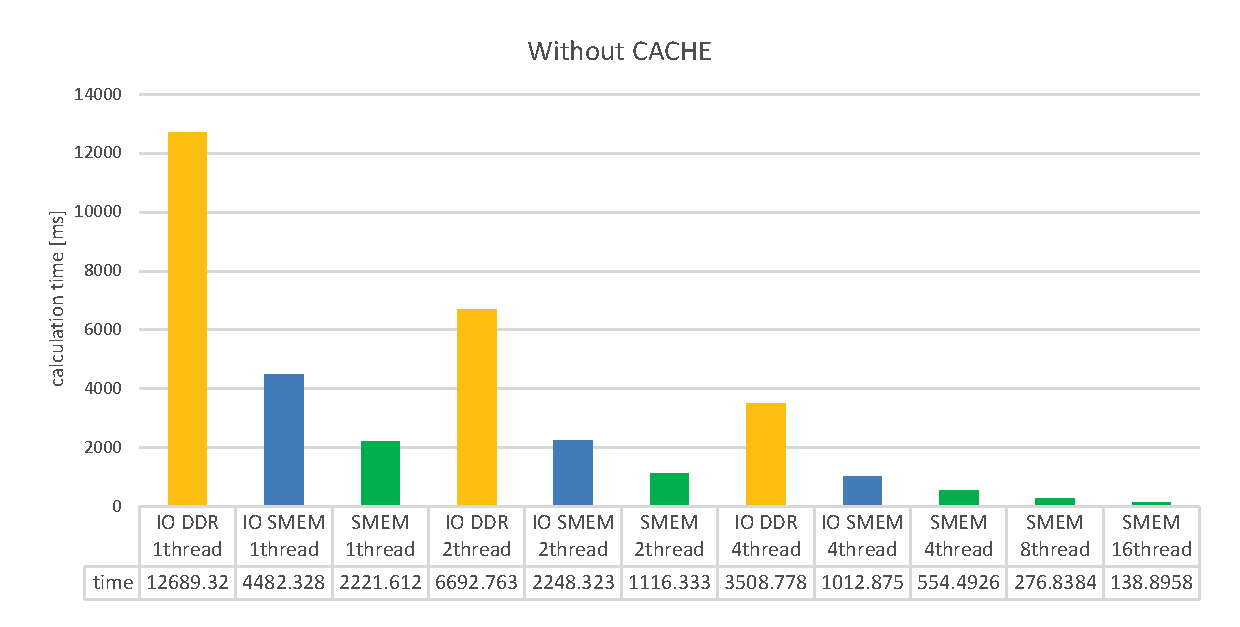
\includegraphics[width=1.0\linewidth]{../figure/BarGraph_matrix_without_cache.eps}
      % \vspace{-7mm}
      \caption{Matrix calculations in IOS and CC without cache.}
      \label{fig:mat_calc_uncash}
    \end{minipage}
    \vspace{-3mm}
  \end{tabular}
  \vspace{-2mm}
\end{figure*}

\subsubsection{Four CCs Parallelization}
\label{sec:four_CCs}
Finally, matrix calculation with offload-computing in IOS and CCs is shown in Figure \ref{fig:mat_calc_offload_314}.
In this case, it is assumed with respect to the calculation of large matrices that the total capacity exceeds 1 MB.
The offloading result is compared with IO DDR (cached) due to the fore-mentioned assumption.
The aggregate calculation is obtained by offloading on the four CC to perform a multiplication of a tile of the transpose of matB and a tile of matC.
This produces a overhead irrespective of the number of threads as shown in Figures \ref{fig:mat_calc_offload_314} and \ref{fig:mat_calc_offload_640}.
However, the speed involved in offloading result exceeds that of IO DDR (cached).
The result indicates several important facts.
First, D-NoC data transfer produces little overhead latency.
Second, the speed of DMA memory access to DDR exceeds that of IO core's memory access.
In the offloading case, a DMA accesses matrix buffers on DDR and transfers the buffers from IO DDR to each CC SMEM.
Subsequently, PEs in the CC access matrix buffer the calculation without cache.
The overhead of data transfer and DMA memory access is small, and thus parallel data transmission and distributed memory are practical in the case of MPPA-256.
The impact of offloading increases when the matrix size is large as shown in Figure \ref{fig:mat_calc_offload_640}.
Only a part of matrix is allocated in CC, and thus it is possible to handle larger matrices buffers.
Additionally, 640 KB matrices are prepared, and matrix calculation calculations are evaluated with offload-computing.
The speed of the offloading result exceeds that of IO DDR result with respect to the 314 KB matrices in Figure \ref{fig:mat_calc_offload_314}.
In these offloading evaluations, each CC concurrently transmits calculation results to the IOS.
When matrix C in which calculation results are stored is allocated in DDR, NoC router's FIFOs sometimes overflow and cause an error.
To avoid this error, matrix C should be allocated in IO SMEM.
Note that above evaluation results when matrix C is allocated in DDR.

\begin{figure*}[t]
  \tabcolsep = 0.5mm              % side-margin in column
  \begin{tabular}{cc}
    \begin{minipage}[t]{0.49\textwidth}
      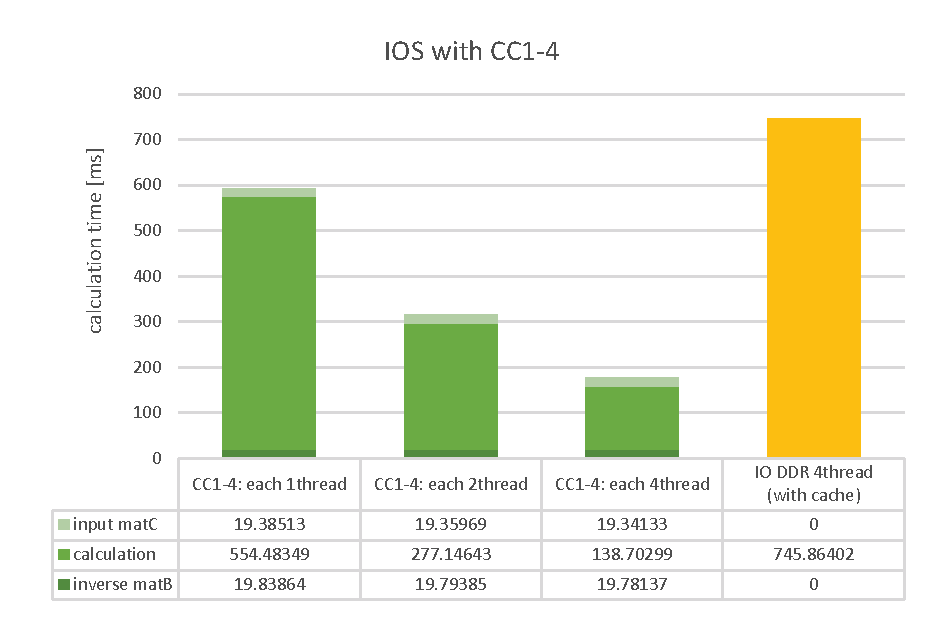
\includegraphics[width=1.0\linewidth]{../figure/BarGraph_matrix_with_CCs_314.eps}
      % \vspace{-7mm}
      \caption{Matrix calculations with offload-computing (314 KB matrix x 3).}
      \label{fig:mat_calc_offload_314}
    \end{minipage}   
    &
    % \setcounter{figure}{11}
    \begin{minipage}[t]{0.49\textwidth}
      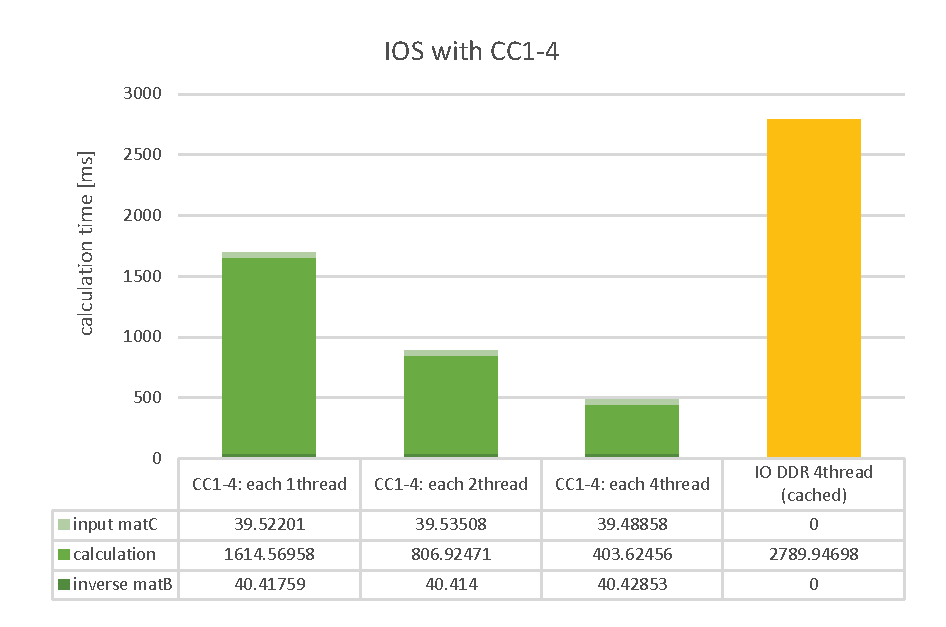
\includegraphics[width=1.0\linewidth]{../figure/BarGraph_matrix_with_CCs_640.eps}
      % \vspace{-7mm}
      \caption{Matrix calculations with offload-computing (640 KB matrix x 3).}
      \label{fig:mat_calc_offload_640}
    \end{minipage}
    \vspace{-3mm}
  \end{tabular}
  \vspace{-2mm}
\end{figure*}

\subsection{Case Study}
\label{sec:case_study}
The application in this case study is a part of an autonomous driving system and this section demonstrates the parallelization potential of the MPPA-256.
We took an algorithm for vehicle self-localization written in C++ in Autoware, namely an open-source software for urban autonomous driving \cite{autoware}, \cite{kato2015open}, and parallelized part of it.
The self-localization adopts the normal-distribution transform matching algorithm \cite{magnusson2009three} implemented in the Point Cloud Library \cite{pcl}.

The self-localization algorithm used in this case study is primarily divided into two processes: \emph{RadiusSearch} which searches for several nearest neighbor points for each query and calculates the distance, and \emph{Derivatives} which calculates the derivative to determine the convergence of the matching operation.
As shown in Figure \ref{fig:ndt_matching_situation}, this evaluation parallelized \emph{Derivatives} onto 16 CCs and the remainder of the algorithm was executed on the IOS.
To parallelize \emph{RadiusSearch}, the algorithm of the nearest neighbor search needs to be redesigned because the data to be searched exceeds 1 MB.
Redesigning this algorithm will be part of a future study..

As shown in Figure \ref{fig:ndt_matching}, the evaluation of parallelized self-localization algorithm indicates the average execution time for each convergence and demonstrates that the parallelization accelerates the \emph{Derivatives} process.
This acceleration shows the parallelization potential of the MPPA-256.
Because the reduction of the execution time of \emph{Derivatives} involves reducing the number of loops for convergence, the execution times of \emph{RadiusSearch} and other parts are also shortened.
The query can be assumed to be 10 Hz in many automated driving systems.
Therefore, if we succeed in the parallelization of \emph{RadiusSearch}, this goal can be achieved.

\begin{figure*}[t]
  \tabcolsep = 0.5mm              % side-margin in column
  \begin{tabular}{cc}
    \begin{minipage}[t]{0.49\textwidth}
      \centering
      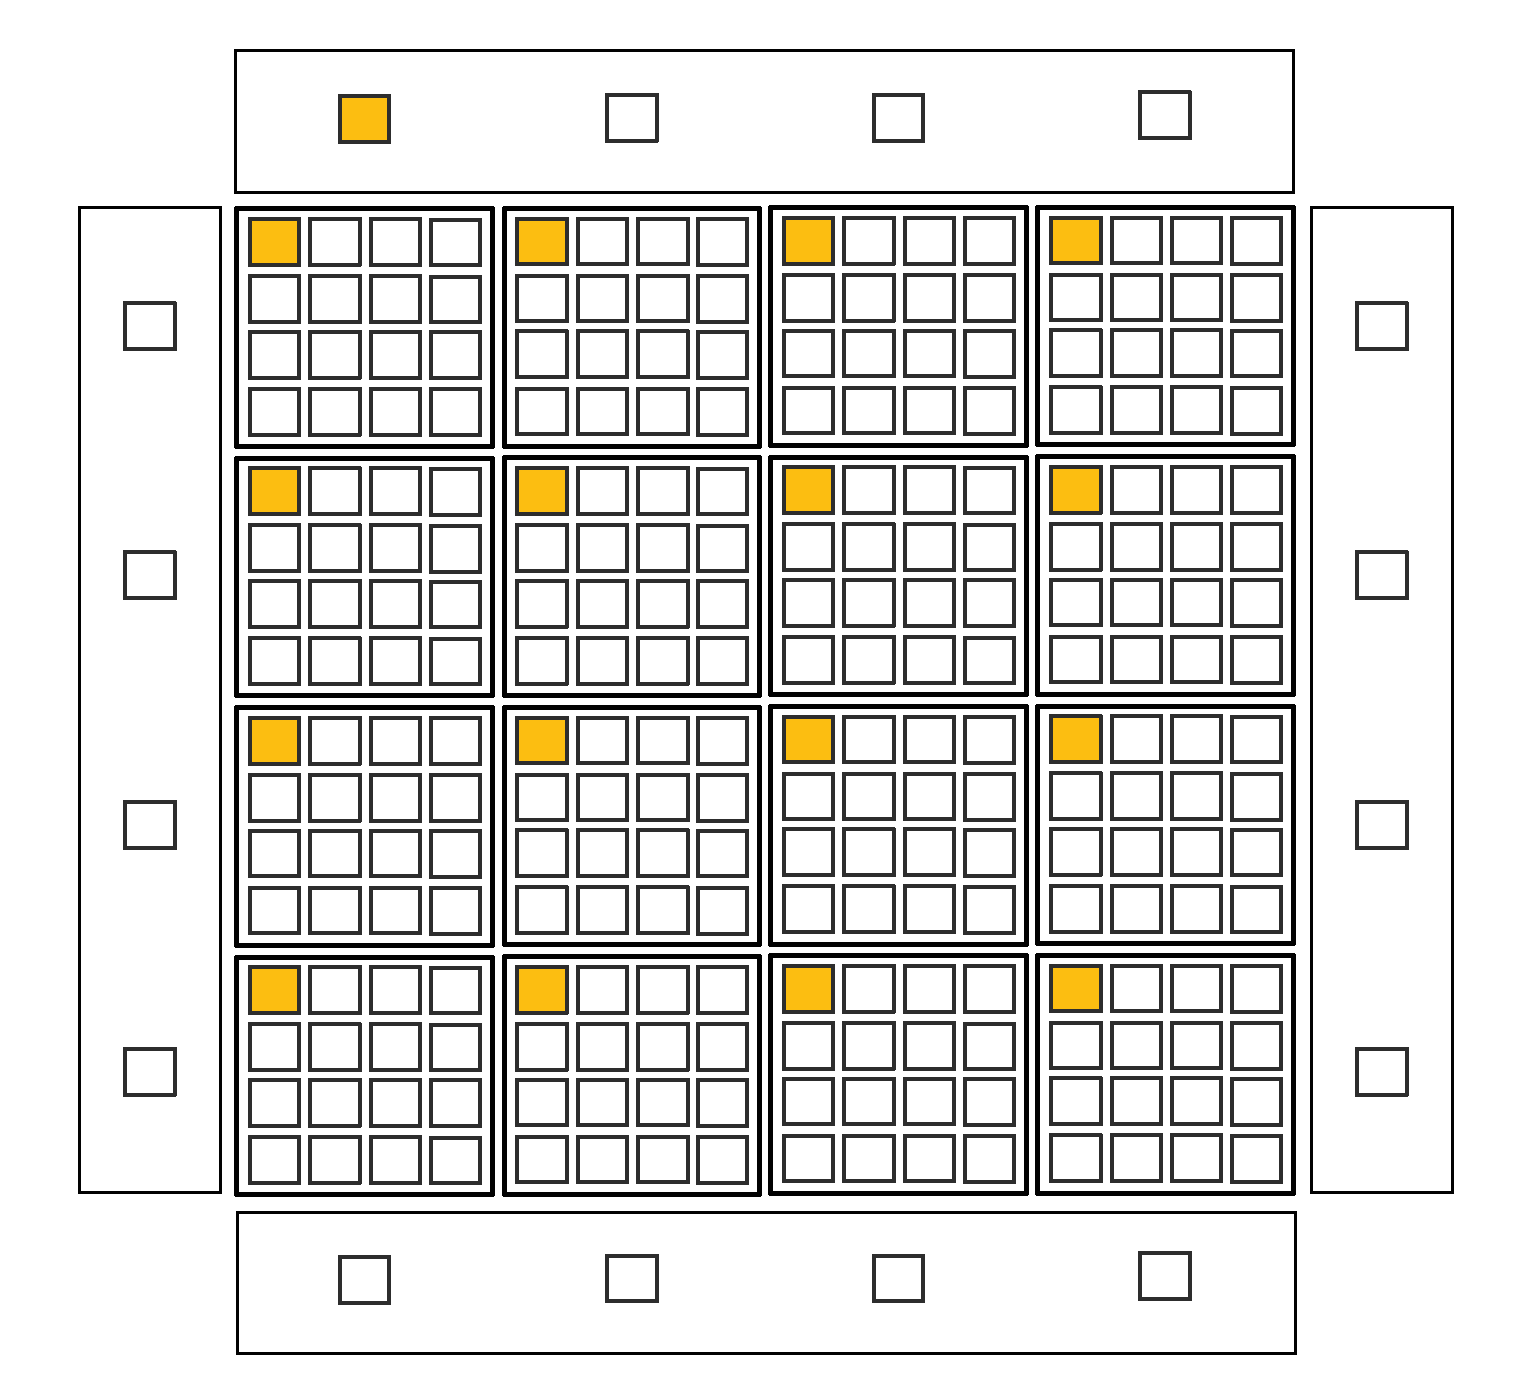
\includegraphics[width=0.7\linewidth]{../figure/ndt_matching.eps}
      \caption{\label{fig:ndt_matching_situation}
      A situation of vehicle self-localization execution.}
    \end{minipage}   
    &
    % \setcounter{figure}{11}
    \begin{minipage}[t]{0.49\textwidth}
      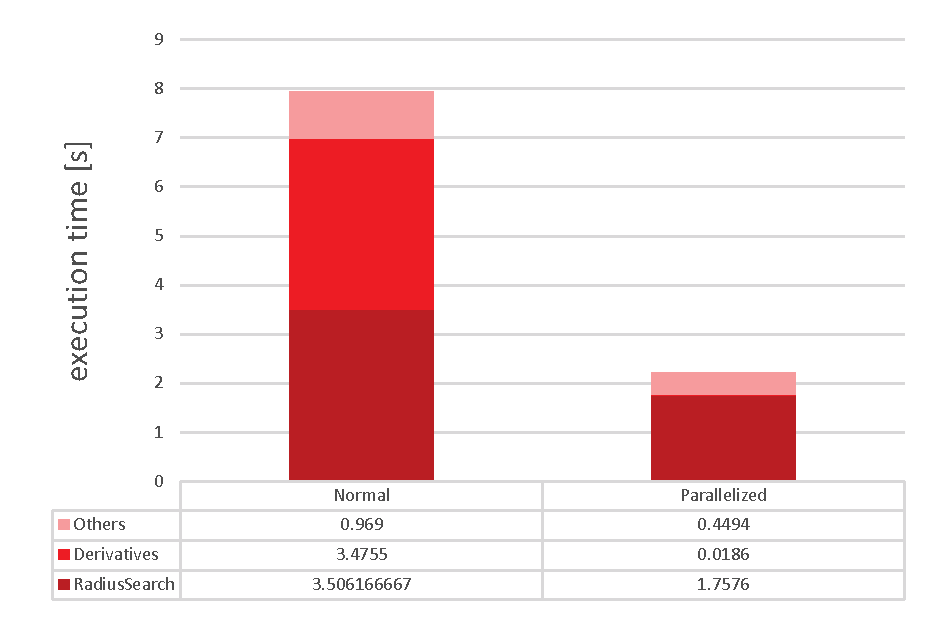
\includegraphics[width=1.0\linewidth]{../figure/BarGraph_ndt_matching.eps}
      \caption{\label{fig:ndt_matching}
      Vehicle self-localization of the partially parallelized autonomous driving application.}
    \end{minipage}
    \vspace{-3mm}
  \end{tabular}
  \vspace{-2mm}
\end{figure*}

\section{Related Work}
\label{sec:related work}
This section compares many-core platforms and discusses previous studies related to multi/many cores.
First, needs of high-performance computation and comparison of many-core platforms to other platforms are discussed.
Second, the Kalray MPPA-256 which this study focuses on is compared to other COTS COTS many/multicore components, and we summarize the features of MPPA-256.
Finally, discussions of previous studies and comparison to them are described.

Recently, studies indicate that the single core processors are characterized by limited computation performance.
Pollack stated that a single core is inefficient \cite{pollack1999new} and that Moore's law \cite{moore2006cramming} is no longer applicable. 
Therefore, extant CPUs are not sufficient to satisfy increasing computation demands.
The shift from a single core in real-Time and embedded systems has occurred \cite{saidi2015shift}. 
Many other platforms including many-core are developed and researched by current studies.

Table \ref{tb:comparison_platforms} summarizes the features of many-core platforms with that of other platforms.
For instance, the GPU is a powerful device to enhance computing performance and it has great potential in specific areas (for e.g., image processing, and learning).
However, it is mainly used for a specific purpose and its reliability is not suitable for real-time systems.
It is difficult to use a GPU for a global purpose and to guarantee its reliability due to the GPU architecture.
Many-core processors based on CPU or DSP cores are significantly superior to GPU with respect to software programmability and timing predictability.
Additionally, it is commonly known that many-core involves a reasonable power consumption.
In contrast, the GPU consumes a significant amount of power and generates considerable heat.
This is a critical problem for embedded systems.
Furthermore, DSPs and FPGAs are also high-performance devices when compared to CPUs.
They are efficient in terms of power consumption.
A DSP is often used for real-time systems and FPGAs guarantee reliability and efficient processing.
They are suitable for time-critical computing \cite{de2015kalray}.
However, DSPs cannot be used for global purpose and programing.
Furthermore, FPGAs are difficult for software developers since their software model is ignificantly different from that of CPU and is not a substitute for CPU.
Many-core platforms can potentially replace single/multi core CPU as they possess ease of programing and scalability with high acceleration.

Based on the fore-mentioned background, many COTS many/multicore components are developed and released by several vendors.
(e.g., Kalray's the Multi-Purpose Processing Array (MPPA) 256 \cite{de2013distributed}, \cite{de2013clustered}, \cite{de2014time}, \cite{baron2010single}, Tilera's Tile-Gx \cite{schooler2010tile}, \cite{ramey2011tile}, Tilera's Tile64 \cite{bell2008tile64}, and Intel's Xeon Phi \cite{chrysos2014intel}, \cite{chrysos2012intel}, Intel's Single-chip Cloud Computer (SCC) \cite{baron2010single}).
The present study focuses on the Kalray MPPA-256 that is designed for real-time embedded applications.
Kalray S.A. \cite{de2013distributed}, \cite{de2013clustered}, \cite{de2014time} presented clustered many-core architectures on the NoC which pack 256 general-purpose cores with high energy efficiency.

MPPA-256 is superior to other COTS many/multicore components in terms of the scalability of the number of cores and the power efficiency as shown in Table \ref{tb:comparison_manycore}.
In terms of the scalability, MPPA-256 adopts 256 cores while other COTS many/multicore components have 64 cores or the number of cores around it.
This scalability of cores is attributed to the memory architecture; each cluster of 16 cores contains its own local shared memory.
The precise hardware model is described in Section \ref{sec:hardware_model}.
When all cores share the global DDR memory as in other platforms excluding MPPA-256, specific bus routes receives extremely large loads and memory access contention frequently occurs.
Local shared memory reduces the above problems and helps the scalability of the number of cores.
This is why MPPA-256 has succeeded in scaling up to 256 cores.
However, the local shared memory architecture restricts the capacity of the memory and requires a data copy from DDR with NoC.
This restriction makes the use of existing applications difficult especially in the case of applications that require more memory.
In terms of power efficiency, MPPA-256 realizes superior energy efficiency despite its large number of cores.
The total clock frequency per watt is the highest of the current COTS many/multicore components.
The power consumption of the MPPA processor ranges between 16W at 600 MHz and 24W at 800 MHz.
While MPPA-256 and TILE64 \cite{bell2008tile64} target the embedded systems, other COTS components consider the HPC accelerator.
Their clock frequency per core exceeds that of embedded solutions.
We need to distinguish the COTS many/multicore components according to their requirements with reference to Table \ref{tb:comparison_manycore}.
MPPA-256 is typically accepted with respect to many-core platforms and the model has been used in several previous studies \cite{perret2016temporal}, \cite{becker2016contention}, \cite{carle2014static}, \cite{perret2016mapping}, \cite{perret2016predictable}.

Several studies have examined real-time applications on many-core platforms including MPPA-256.
In Ref. \cite{saidi2015shift}, multiple opportunities and challenges of many/multicore platforms are discussed.
The shift to many/multicore in real-time and embedded systems is also described. 

Based on the above background, several task mapping algorithms for many/multicore systems have been proposed \cite{perret2016mapping}, \cite{puffitsch2015off}, \cite{carle2014static}, \cite{becker2014mapping}, \cite{faragardi2014communication}.
Airbus S.A.S. \cite{perret2016mapping} proposes a method of directed acyclic graph (DAG) scheduling for hard real-time applications using MPPA-256.
In Ref. \cite{faragardi2014communication}, a mapping framework is proposed on the basis of AUTOSAR which is applied as a standard architecture to develop automotive embedded software systems \cite{furst2009autosar}.
AUTOSAR task scheduling considering contention in shared resources is presented in Ref. \cite{becker2016contention}.

By examining the above mapping algorithms of real-time applications, several previous studies \cite{kanter2015kalray}, \cite{denet2017work}, \cite{deDinechin2014GSN}, \cite{perret2016predictable} have analyzed the potential of MPPA-256 and data transfer with NoC as shown in Table \ref{tb:comparison_relatedwork}.
MPPA-256 is introduced, and its performance and energy consumption are reported in Ref. \cite{kanter2015kalray}.
However, this report contains few evaluations and does not refer to data transfer with NoC and memory access characteristics.
Data transfer with NoC in MPPA-256 is described, and NoC guaranteed services are analyzed in Refs. \cite{denet2017work} and \cite{deDinechin2014GSN}.
While the theoretical analysis is thorough in these studies, the practical evaluations are poor and parallel data transfer is not referred to.
The authors of Ref. \cite{perret2016predictable} focused on the predictable composition of memory accesses.
An analysis of their study identified the external DDR and the NoC as main bottlenecks for both the average performance and the predictability on platforms such as MPPA-256.
Although the analysis examined the memory access characteristics of the external DDR and provided notable lessons, a solution for the DDR bottleneck was not examined and practical evaluations were lacking.

% \renewcommand{\arraystretch}{1.2}
\begin{table*}[t]
  \caption{\label{tb:comparison_platforms}
    Comparison of Many-core to CPU, GPU, DSP, and FPGA}
  \centering
  \scriptsize	                    % text size
  \tabcolsep = 1.5mm              % side-margin in column
  \begin{tabular}{c|cccccccccc}
    \hline
    & \multirow{2}{*}{performance} & \multirow{2}{*}{power/heat} & \multirow{2}{*}{reliability} & \multirow{2}{*}{real-time} & software & \multirow{2}{*}{costs} & multiple\\
    &&&&& development && instruction \\
    \hline
    \hline
    CPU & & \(\bigtriangleup\) & \(\checkmark\) & \(\checkmark\) & \(\checkmark\) & \(\checkmark\) & \(\bigtriangleup\) \\
    GPU & \(\checkmark\) &  & \(\bigtriangleup\) &  & \(\bigtriangleup\) & \(\checkmark\)\\
    DSP & \(\bigtriangleup\) & \(\bigtriangleup\) & \(\checkmark\) & \(\checkmark\) & \(\bigtriangleup\) & \(\checkmark\) & \\
    FPGA & \(\checkmark\) & \(\bigtriangleup\) & \(\checkmark\) & \(\bigtriangleup\) &  & \(\bigtriangleup\) & \\
    Many-core & \(\checkmark\) & \(\checkmark\) & \(\checkmark\) & \(\checkmark\) & \(\checkmark\) & \(\bigtriangleup\) & \(\checkmark\) \\
    \hline
  \end{tabular}
  \vspace{-5mm}
\end{table*}

% \renewcommand{\arraystretch}{1.2}
\begin{table}[t]
  \caption{\label{tb:comparison_manycore}
    Comparison of Many-core Processor Platforms}
  \centering
  \scriptsize	                    % text size
  \tabcolsep = 1.5mm              % side-margin in column
  \begin{tabular}{c|cccc}
    \hline
    & \multirow{2}{*}{scalability} & power  & code & \\
    & & efficiency & transplant & \\
    \hline
    \hline
    Kalray MPPA-256 \cite{de2014time} & \(\checkmark\) & \(\checkmark\) & \(\bigtriangleup\) & \\
    Tilera Tile series \cite{bell2008tile64} &  & \(\bigtriangleup\) & \(\checkmark\) & \\
    Intel Xeon Phi \cite{chrysos2014intel} \cite{chrysos2012intel} &  &  & \(\checkmark\) & \\
    Intel SCC \cite{baron2010single} &  &  & \(\checkmark\) & \\
    \hline
  \end{tabular}
  \vspace{-5mm}
\end{table}

% \renewcommand{\arraystretch}{1.2}
\begin{table*}[t]
  \caption{\label{tb:comparison_relatedwork}
    Comparison of Related Work}
  \centering
  \scriptsize	                    % text size
  \tabcolsep = 1.5mm              % side-margin in column
  \begin{tabular}{c|ccccccccc}
    \hline
    & performance & data transfer & memory access & \multirow{2}{*}{real applications} & parallel data & \\
    & analysis & analysis with NoC & characteristics & & transfer & \\
    \hline
    \hline
    Kalray clusters calculate quickly \cite{kanter2015kalray} & \(\bigtriangleup\) &  &  &  &  & \\
    Network-on-Chip Service Guarantees \cite{denet2017work} &  & \(\checkmark\) &  &  &  & \\
    Predictable composition of memory accesses \cite{perret2016predictable} &  & \(\checkmark\) & \(\checkmark\) &  &  & \\
    this paper & \(\checkmark\) & \(\checkmark\) & \(\checkmark\) & \(\checkmark\) & \(\checkmark\) & \\
    \hline
  \end{tabular}
  \vspace{-5mm}
\end{table*}


\section{Conclusions}
\label{sec:conclusion}
This paper has conducted quantitative evaluations that examined end-to-end latencies with many-core computing based on NoC, the scalability of parallelization, and the characteristics of the memory access speed.
From various experiments, we have evaluated the capabilities of the currently available data transfer methods and the parallelization potential for many-core computing based on NoC.
Our experimental results will allow system designers to choose appropriate system designs based on the requirements of their latency-sensitive many-core applications beyond an intuitive expectation.

In future studies, we will port real-time systems software such as that in Ref. \cite{maruyama2016ros2} and propose the parallelization of memory intensive algorithms such as the nearest neighbor search in Section \ref{sec:case_study}.


\section{acknowledgements}
\label{sec:acknowledgements}
We acknowledge support from eSOL and Kalray.
The authors would like to thank Atsushi Matsuo and Masaki Gondo from eSOL, and Gilbert Richard, Stéphane Cordova, and Benoît De Dinechin from Kalray for their support that helped improve this study.

%%
\bibliographystyle{abbrv}       % ACM
\bibliography{reference}

\end{document}

